\documentclass[a4paper,11pt]{article}
\usepackage[margin=2cm]{geometry}
\usepackage{graphicx}
\usepackage{color, colortbl}
\usepackage{cite}
\usepackage{url}
\usepackage{float}
\usepackage{arydshln}
\usepackage{pdfpages}
\usepackage{csvsimple}
\usepackage{listings}
\usepackage{algpseudocode}
\usepackage{longtable}
\usepackage{pdflscape}

\definecolor{Green}{rgb}{0.6,1,0.6}
\definecolor{Amber}{rgb}{1,1,0.4}
\definecolor{Red}{rgb}{1,0.6,0.6}

\usepackage{fancyhdr}
\pagestyle{fancyplain}
\fancyhf{}
\lhead{\fancyplain{}{M.Sc.\ Group Project Report}}
\rhead{\fancyplain{}{\today}}
\cfoot{\fancyplain{}{\thepage}}

\title{Plant Recognition: Bringing Deep Learning to iOS\\\Large{--- Final Report ---}}
\author{Cutmore Ashley, Dalyac Alexandre, Douglas Stewart,\\ Haughian Gerard, Leigh Simon, McCormac John\\
       \{ac7513, ad6813, sd3112, gh413, sjl213, bjm113\}@ic.ac.uk\\ \\
       \small{Supervisor: Dr William Knottenbelt and Mr Jack Kelly}\\
       \small{Course: CO530/533, Imperial College London}
}

\begin{document}

\maketitle

\abstract
{
Automatic species recognition of plants in natural scenery is an unmet challenge with considerable user demand from the smartphone app market. LeafSnap, developed by Columbia University's machine vision lab, has attracted 150,000 downloads but has received poor reviews due to its inability to deal with cluttered backgrounds and within-class variance. We propose WhatPlant, an iOS App powered by a cutting edge convolutional neural network to overcome LeafSnap's shortcomings. We achieve a 29\% top-5 classification accuracy on 259 plant species, with images of plants taken in natural scenery. This report accompanies the official release of our App on Apple's App Store, and sets out the implementation of our work from beginning to end.
}

\clearpage
\tableofcontents
\clearpage

\section{Introduction}

Accurate and portable plant identification has many motivations: the pragmatic farmer identifying a weed, families in the park curious about their natural surroundings, conservationists keen to gather accurate botanical data, citizen science projects for the control of invasive species. For a human to visually identify plants requires years of specialised training, but recent advances in computer vision and artificial intelligence make it possible to take a machine through comparable training in a matter of days. This opens the possibility of enabling anybody with a smartphone to identify plants with a reasonable degree of accuracy, and allow such data collection and analysis to be available to non-experts en masse.

This report describes the creation of an iOS app for recognising plant species based on images taken in natural scenery. The project is divided into three components: an iOS app front-end, a server system to enable communication between the app and our classifier, and a Convolutional Neural Network to classify the images. This report takes the reader through the following sections, each of which branch off into the three project components:
\begin{itemize}
 \item \textbf{Specification} : The original outline of the project, our interpretation of it, and the specific tasks we set for ourselves.
 \item \textbf{System Architecture} : An overview describing how the three components of our product fit together and interact.
 \item \textbf{Product Design} : The look and feel of our product to the user.
 \item \textbf{Methodology} : Our production development strategy, including unit testing.
 \item \textbf{Implementation} : The biggest challenges we encountered and how we dealt with them.
 \item \textbf{Final Product} : Evaluation of the performance of our product, and the commercial opportunities it presents.
\end{itemize}
 
Overall, the project presented ambitious goals - since, to our knowledge, no app for recognising plants in natural scenery exists - but the goals were met: our app can classify 259 plant species with 29\% top-5 accuracy, and is currently being downloaded and used by iOS users on Apple's App store.

\clearpage
\section{Specification}

\subsection{Original Specification}


%Specification of the functionality that your project aims to provide. The contents of this section would normally be provided by Report One. In addition to that, explain whether you had to make any changes to the original requirements, and why (this may be taken from Report Two).%

The original proposal stated that ``The ultimate aim is to produce a smart phone application which can automatically identify a plant from a photo''. There already exists an iOS app which promises to do this \cite{leafsnap_scientificamerica} - but only if supplied with a photo of a leaf against a white background. Hence, our key objective became the production of an improved alternative that addresses the weaknesses of the existing solution.

The original proposal considered three areas for development: the smartphone application, the server and the classification engine. Two different directions were suggested for the classification engine: manually writing feature detectors, or automatic detection of features (i.e. machine learning). Possible features and implementation details were proposed such as uploading a group of images per classification, linking results to 3rd party reference sites e.g Wikipedia and server job queue management.

\subsection{Interpretation}

With a very broad and open specification the first item on our agenda was to give the project a focused direction that we felt minimised compromise, was achievable and got us excited. Group meetings, discussions with our project supervisors and a system of Goal-Orientated Capture [Figure~\ref{fig:goalorientedcapture}] allowed us to come to a mutual understanding of the specific goals of the project. 

\begin{figure}[h!]
  \centering
  %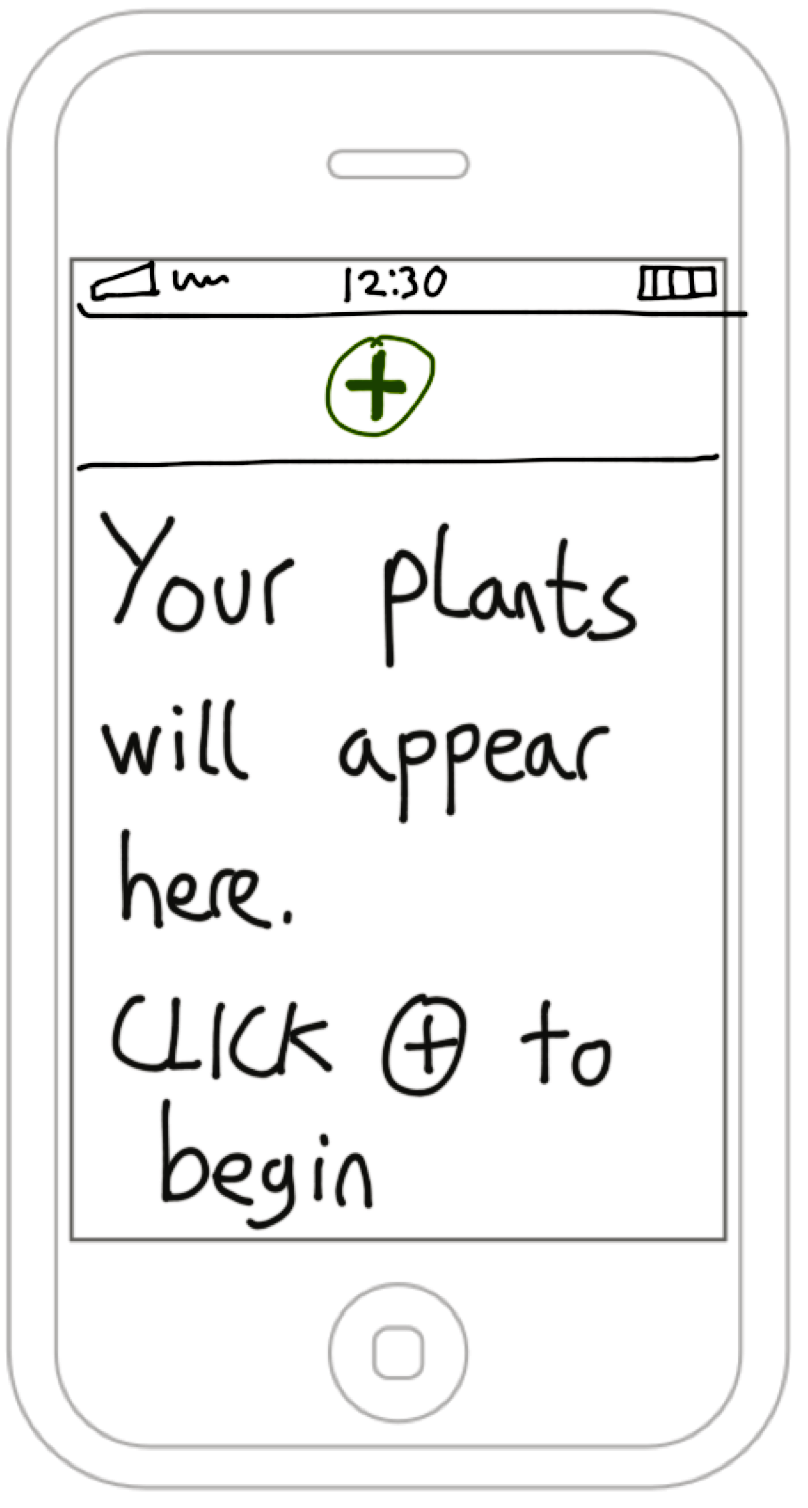
\includegraphics[width=0.22\linewidth]{BeLeaf1.png}
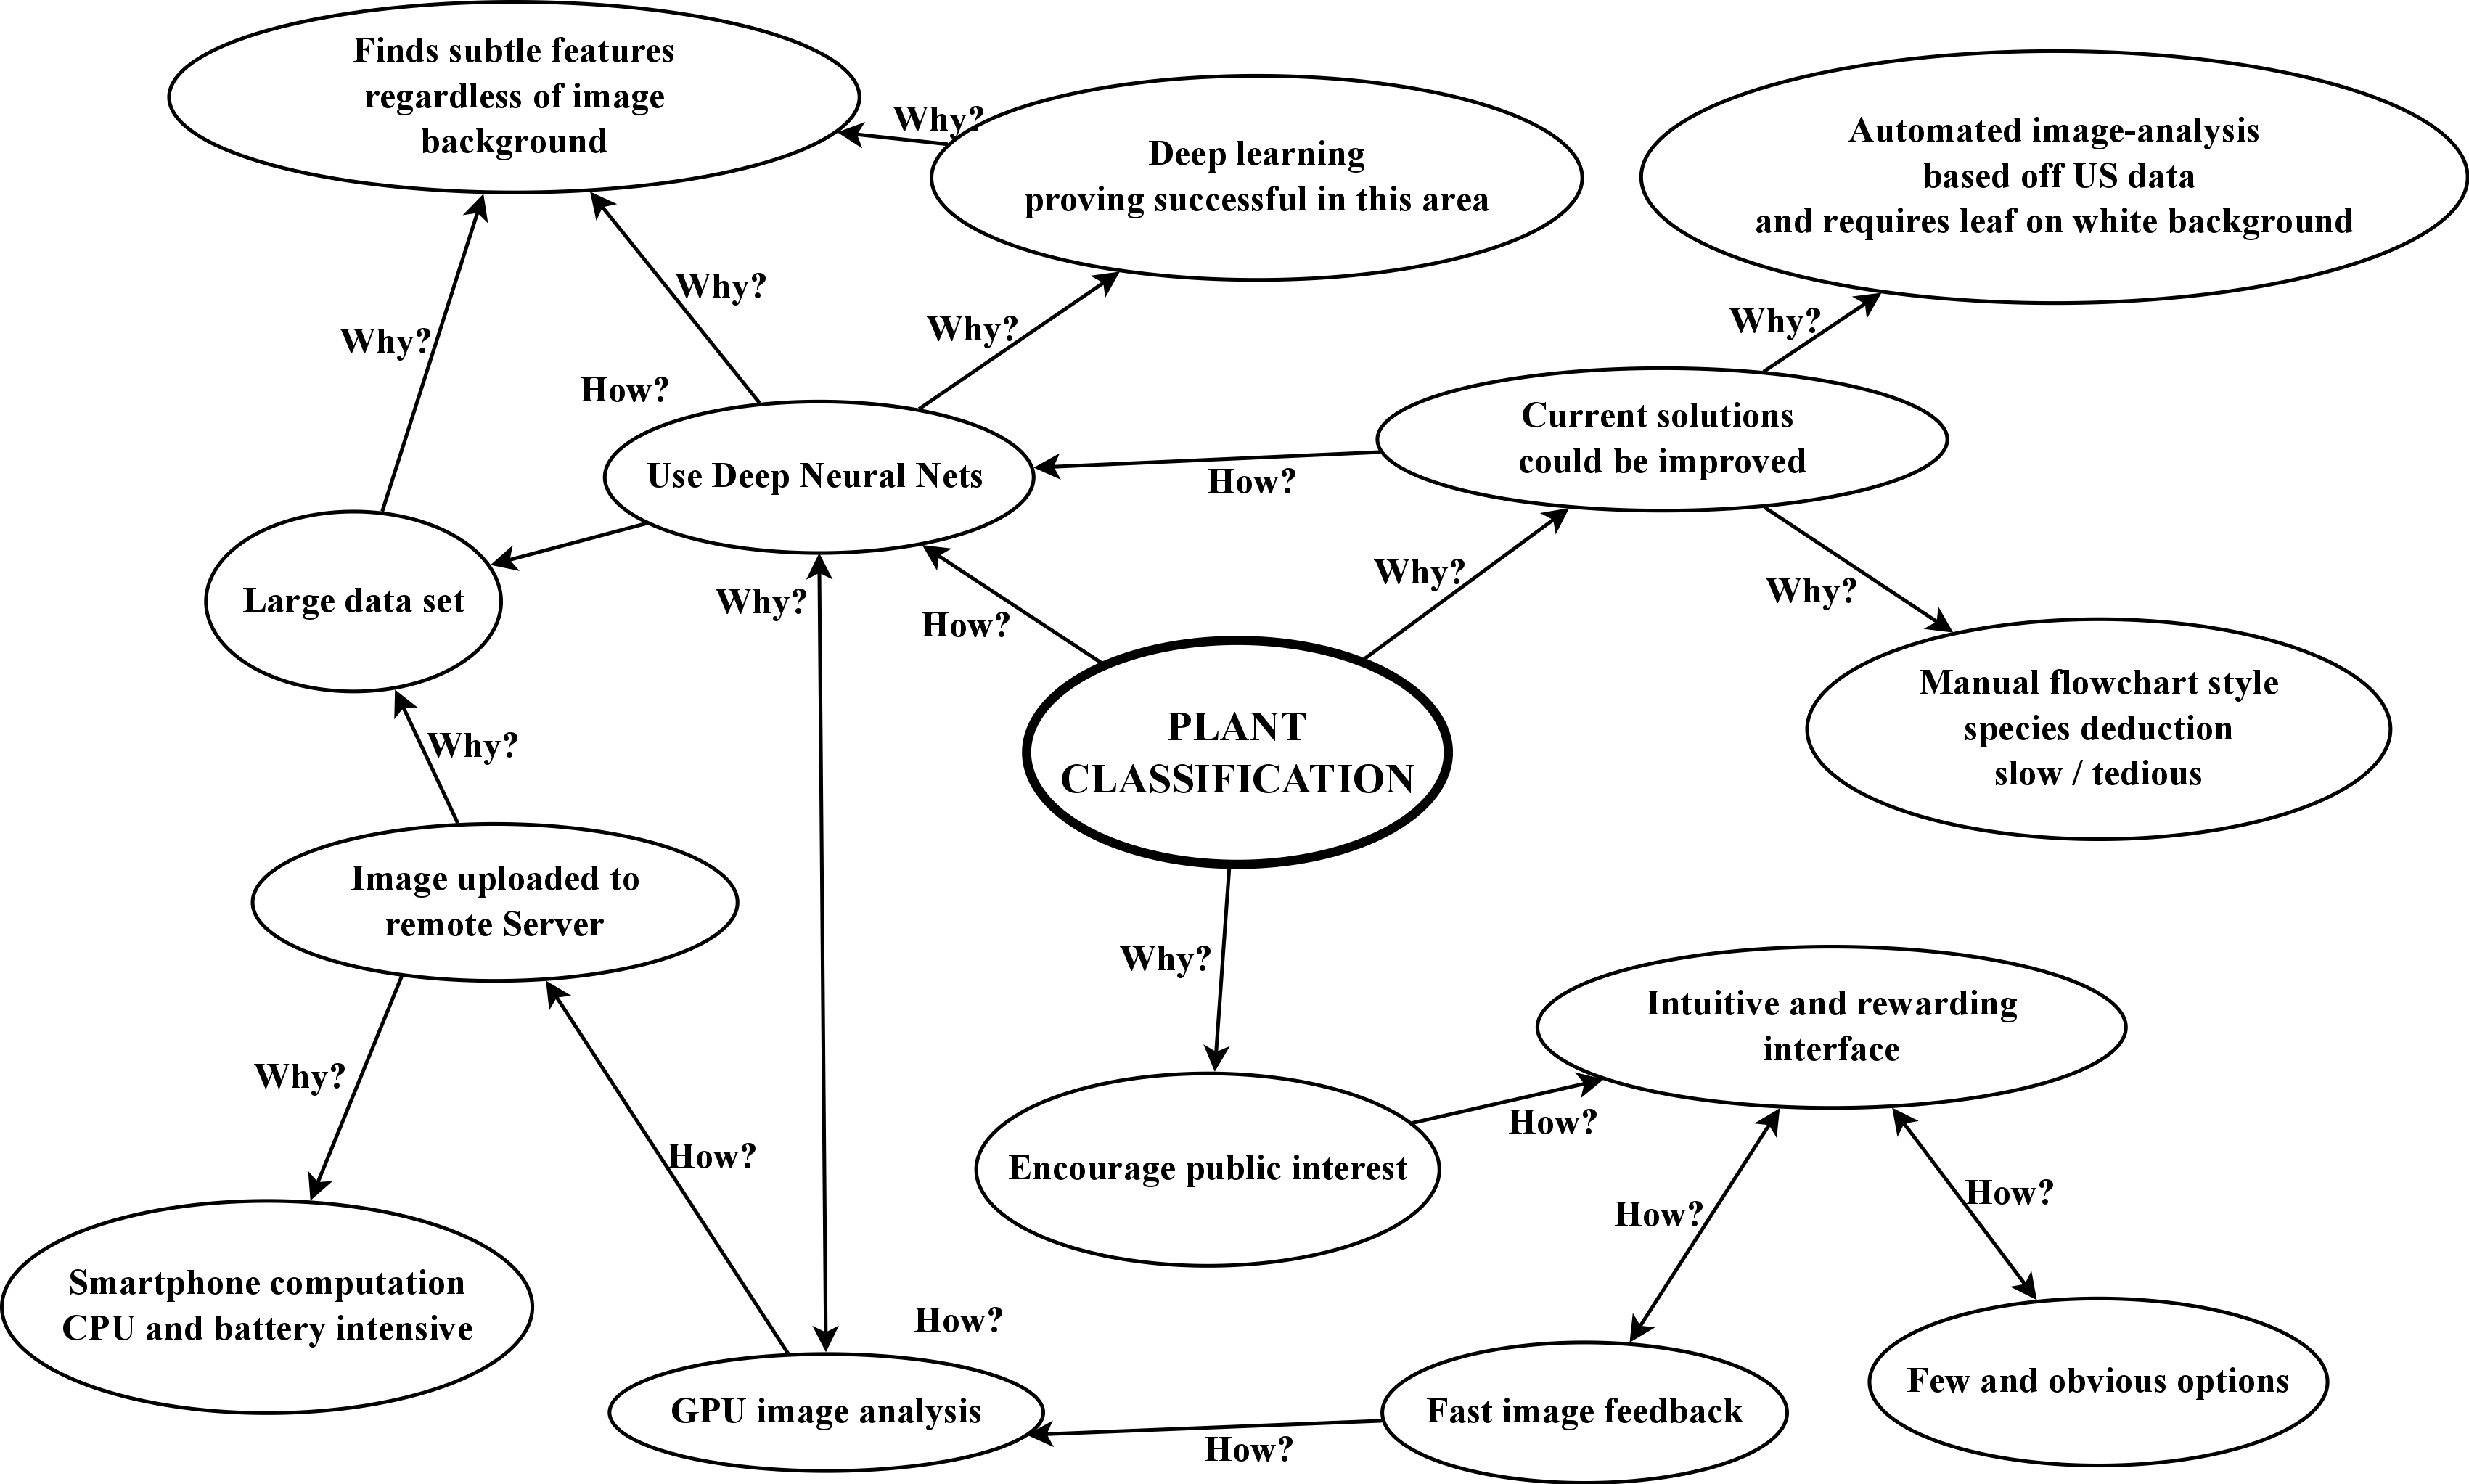
\includegraphics[width=165mm]{images/plantclassgoalcapture.png}
  \caption{Goal-Orientated Capture}
  \label{fig:goalorientedcapture}
\end{figure}

Central to this project is software enabling accurate and automatic identification of a plant from a single or multiple images of the plant (leaf, flower, fruit, or the entire specimen) in its natural environment.  Ideally, the process of identification should not require manipulation of the plant or its surroundings and should also only take a short period of time (on the order of seconds). To achieve this we took a deep learning approach using Alex Krizhevsky's cuda-convnet which utilises the GPU available to us during the project.

The smartphone app was developed for iOS7 and designed to be intuitive to use: leading a user naturally from taking a photo to an understandable result. The server maintains a database of jobs and results, and communicates with the app using HTTP.

To help the team structure the project we translated the above goals into sets of deliverables for each of the project's three main areas: iOS Application, Plant Classification, and Server. We have differentiated these deliverables across two dimensions. Firstly, we assigned them to either an Essential or Supplementary category. Essential deliverables were seen as key to the project's success, whereas Supplementary deliverables typically represent additional features that could be added. Secondly, each deliverable is given a High, Medium or Low priority to help the team plan the project's time-line. Each deliverable and its corresponding category and priority is listed below. Deliverables that were were added after the original goal capture meeting are highlighted.(with a Category `$+$'). In the tables below, we show the final state of each deliverable and the estimated completion date (ECD).\\

\subsubsection{iOS 7 Application}

\begin{table}[H]
\small
\centering
\begin{tabular}{ c p{11cm} c c c }
  Cat & Description & Priority & ECD & Status\\
  \hline
  E & \textbf{iOS 7 application that can take and store photos.} & H & Sprint1 & Complete\\
  E & \textbf{Application can upload photos to server.} & H  & Sprint1 & Complete \\
  E & \textbf{Application can receive and handle classification result from server.} & H & Sprint1 & Complete\\
  E & \textbf{Classification result can be displayed to user.} & H & Sprint1 & Complete \\
  S & \textit{Photo geographical location stored.} & L & Sprint1 & Complete \\  
  S & \textit{HTML5 web interface available for desktop and non-iOS mobile.} & M & Sprint3 & Removed\\
  S & \textit{Link to web (e.g. Wikipedia) entry for species.} & M  & Sprint3 & Complete\\
  S & \textit{Application released on Apple's App Store.} & M & Sprint3 & Complete \\
  S & \textit{Comparison image displayed.} & M & Sprint3 & Removed \\
  S & \textit{User feedback of result returned to server.} & L & Sprint3 & Removed \\
  \hdashline
  $+$ & \textbf{User can select one of four plant components (e.g. Leaf, Fruit, Flower) to improve result accuracy.} & - & Sprint3 & Complete \\
\end{tabular}
\end{table}

%\newpage
\subsubsection{Plant Classification}

\begin{table}[H]
\small
\centering
\begin{tabular}{ c p{11cm} c c c}
  Cat & Description & Priority & ECD & Status \\
  \hline
  E & \textbf{A neural network that processes an image and returns a classification.} & H & Sprint1 & Complete \\
  E & \textbf{Neural network capable of handling required image resolution.} & H & Sprint1 & Complete \\
  E & \textbf{Determine image resolution that produces a relevant result.} & H & Sprint1 & Complete \\
  E & \textbf{Interface integrated with the rest of the system.} & H & Sprint1 & Complete \\
  E & \textbf{Result produced within an acceptable time interval.} & M & Sprint2 & Complete \\
  E & \textbf{Acceptable classification time for users determined.} & M & Sprint2 & Complete \\
    S & \textit{Image manipulation scripts to augment training set.} & M & Sprint2 & Complete \\
  S & \textit{Neural network capable of processing multiple images for a single plant.} & M & Sprint3 & Complete \\
  \hdashline
  $+$ & \textbf{A neural net to retag ImageNet data by plant component type.} & - & Sprint2 & Complete\\
  $+$ & \textbf{A training database with taxonomical bucketing algorithm.} & - & Sprint2 & Complete \\
\end{tabular}
\end{table}

\subsubsection{Server}

\begin{table}[H]
\small
\centering
\begin{tabular}{ c p{11cm} c c c}
  Cat & Description & Priority & ECD & Status\\
  \hline 
  E & \textbf{Define RESTful interface allowing image and image meta-data to be received from iOS 7 application and response delivered from server.} & H & Sprint1 & Complete \\
  E & \textbf{Define interface between application-facing server and plant classification software.}  & H & Sprint1 & Complete \\
  E & \textbf{Classification requests forwarded to our neural network for processing.} & H & Sprint1 & Complete\\
  E & \textbf{Classification results received back from the neural network.} & H & Sprint1 & Complete \\
  E & \textbf{Plant classifications stored in database.} & H & Sprint1 & Complete \\
  E & \textbf{Classification passed back to user/iOS 7 application.} & H & Sprint1 & Complete \\
  E & \textbf{Plant images and appropriate meta-data stored in database.} & M & Sprint1 & Complete \\
  E & \textbf{Basic queue for requests implemented.} & M & Sprint1 & Complete \\
  S & \textit{Images hashed and stored in database.} & L & Sprint2 & Removed \\ 
  S & \textit{Requests can be sent to multiple neural networks.} & L & Sprint3 & Removed \\
  S & \textit{Open API provided for 3rd parties to interact with our backend.} & L & Sprint3 & Removed\\
  S & \textit{Hashed image used to check previous uploads of same image.} & L & Sprint3 & Removed \\
  S & \textit{Duplicate images not stored or re-processed.} & L & Sprint3 & Removed \\
  S & \textit{Requests to connect to server authenticated.} & L & Sprint3 & Removed \\
  S & \textit{Stored classification results returned on hash collision.} & L & Sprint3 & Removed \\
  S & \textit{Result accuracy tracked over classification versions.} & L & Sprint3 & Removed \\
  \hdashline
  $+$ & \textbf{Separate `Worker' server executes combine script when all images of plant received.} & - & Sprint3 & Complete \\
\end{tabular}
\end{table} 

\subsection{Changes to Original Specification}

\subsubsection{Added}

\begin{itemize}
  
 \item \textbf{User can select one of four plant components (e.g. Leaf, Fruit, Flower) to improve result accuracy.}
 
 Given the disparate nature of features between images (consider a flower vs. a leaf), we felt that training separate smaller neural networks on each of the components could improve classification performance. This motivated us to allow the user to capture four different components of each specimen.
 
  \item \textbf{A neural network to retag ImageNet data by plant component type.}
  
  The ImageNet data we had was tagged by species, but not by `component type' (i.e. Leaf, Fruit, Flower, Entire). We overcame this issue by using an alternate dataset (provided by PlantClef \cite{plantclef}, which did have these tags) to train a separate neural network to tag each of our two million images from ImageNet, before inserting it into our training database.
  
  \item \textbf{A training database with taxonomical bucketing algorithm.}
  
  The motivation for this bucketing algorithm was to ensure our neural network wasn't burdened having to learn to recognise species for which we had a limited training subset (i.e. few images of an individual species). Bucketing those images into a higher level in our taxonomy tree meant we could decrease our neural network error rate while maximising our use of available training data. We wrote a bucketing algorithm which could dynamically bucket plant species into buckets which contained a minimum threshold of images which could be classified based on a taxonomy tree we constructed using WordNet\cite{wordnet}. 
 
   
   \item \textbf{Separate `Worker' server executes combine script when all images of plant received.}
   
   To ensure modularity and scalability of our architecture, it was decided early in Sprint 1 to create independent `Request' and `Worker' servers. These servers run on  distributed machines and both connect to the same database.
   
\end{itemize}
\clearpage
\subsubsection{Removed}

\begin{itemize}
\item \textbf{User feedback of result returned to server.}
  
  It was noted in our meeting with the Natural History Museum that the general public often misclassified plants, and that even experts regularly misclassified. Thus, we removed crowd-sourced classifications from the iOS application because it was felt that it cluttered the design and would not add to our classification accuracy. 
  
     \item \textbf{Image Hashing and Duplicate Image Detection}
   
   The changes to the iOS application made hashing uploaded images unnecessary. The application does not allow users to upload the same image twice.
   
   \item \textbf{HTML5 Interface and API}
   These were omitted as they were non-essential and it was felt that development time would be better spent on the other deliverables.
  
\end{itemize}
     


\subsection{Revised Schedule}

There was one major, unforeseen issue in Sprint 1 which caused a significant impact on our original proposed schedule. This also affected later Sprints: the main source for our neural network training data, ImageNet, experienced technical difficulties with their web site; causing it to be inaccessible for a full week. Once the site was available again, we then were further delayed for five full days downloading a 1.2TB tar file of images. This too impacted our ability to progress with many Plant Classification tasks for Sprint 1. All other tasks proceeded as scheduled, taking into account revised goals as iterations of the product were developed.


\clearpage
\section{System Architecture}

The specification presented two essential features for our architecture: an iOS app and a `Worker' server capable of classifying images sent to it. In particular, the Worker server needed to have a powerful GPU to support NVIDIA's CUDA platform \cite{nvidiacuda}. To help us complete our project, the Computing Support Group provided us with a dedicated lab machine with a powerful GPU.

A number of different configurations were discussed initially, including having the iOS app communicate directly with the Worker server, which itself would be linked to a data store. However, this early proposal was rejected as it could not scale effectively. Instead, the final architecture includes a `Request' server, which acts as an intermediary between the iOS app and the Worker server. If the app becomes popular then this would allow us to distribute the image classification tasks across a number of different Worker servers. 

The Request server runs on a virtual machine and communicates with the iOS app using HTTP GET, POST and PUT requests. To store the metadata associated with each image we use the MongoDB NoSQL document database, because it can scale rapidly and executes reads and writes quickly. Furthermore, our data is not strongly `relational', meaning an SQL solution was not necessary. The MongoDB database runs on the Request server but is accessible from the Worker server. 

Upon receiving an image from the iOS application, the Request server modifies our MongoDB collections and forwards the image to the Worker server. Concurrently, the Worker server is polling the database for unclassified images, which it then runs through our neural network. Finally, when all the images of a certain plant have been analysed, the results are aggregated using our Bayesian Classifier. The iOS application is then responsible for requesting results.


\begin{figure}[h!]
  \centering
  %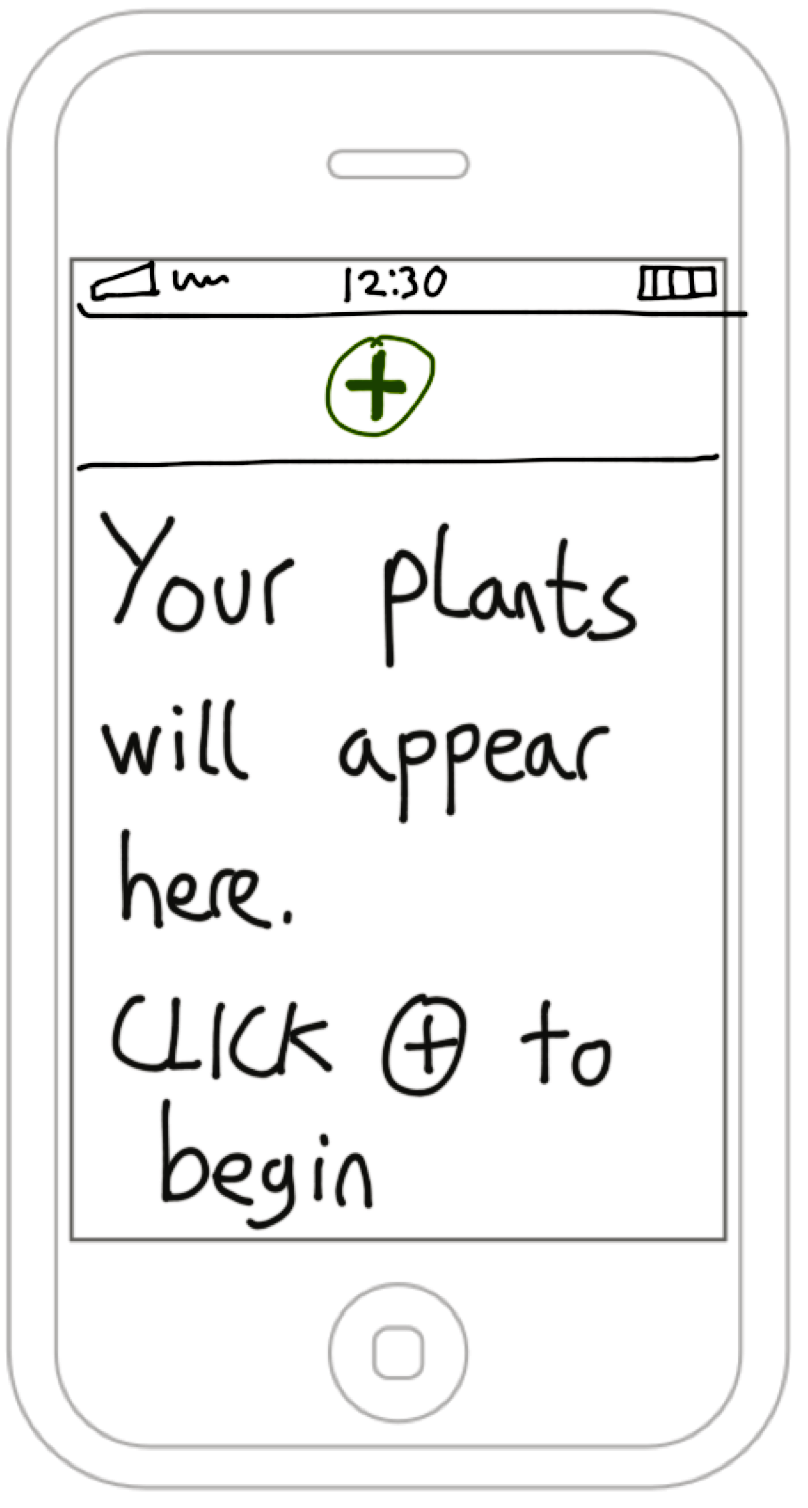
\includegraphics[width=0.22\linewidth]{BeLeaf1.png}
  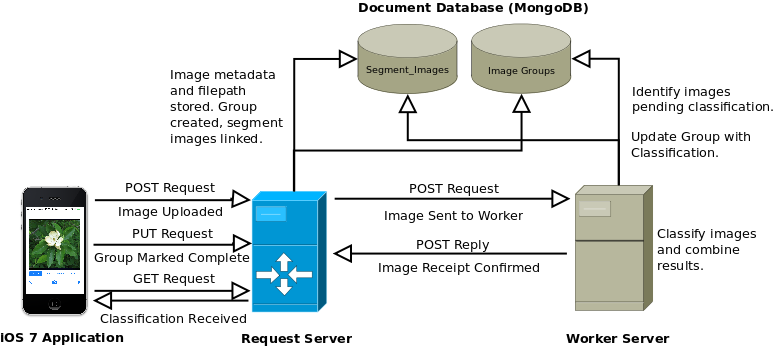
\includegraphics[width=1\linewidth]{SystemContextDiagram.png}
  \caption{System Context Diagram}
  \label{fig:systemcontextdiagram}
\end{figure}

\clearpage

\section{Product Design}

The design of the product will determine the user's experience of using our software long before a result is shown. A prototype application was built during the first sprint that could take images, upload these to the server and receive and display a result. This was made possible by the organisation of `protocol meetings', to specify the interface between the application and the server.  In an extensive UI design session during sprint 2 we prototyped different interface work-flows, sketching ideas onto paper wire-frames. As we planned to release on the App Store, our designs had to stay aligned with Apple's detailed guidelines. The user interface was simplified to minimise the options available to the user and we reduced each classification session to three views: Home, Capture and Review. An initial version of the updated design was completed by the end of Sprint 3. In this version, photos can be taken and reviewed for different plant components before being saved and uploaded in the background during one continuous camera session. 

\begin{figure}[h!]
	\centering
	%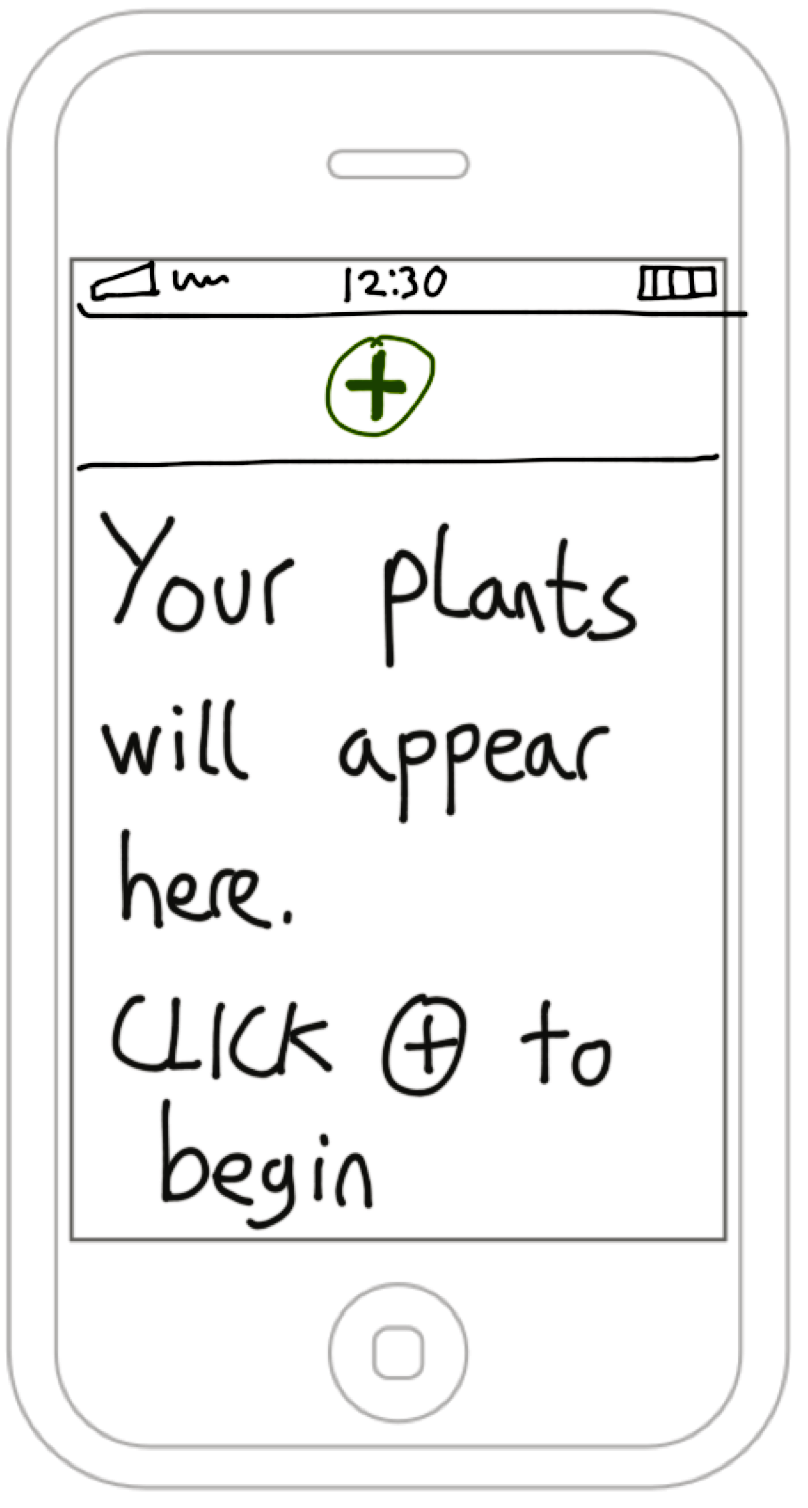
\includegraphics[width=0.22\linewidth]{BeLeaf1.png}
	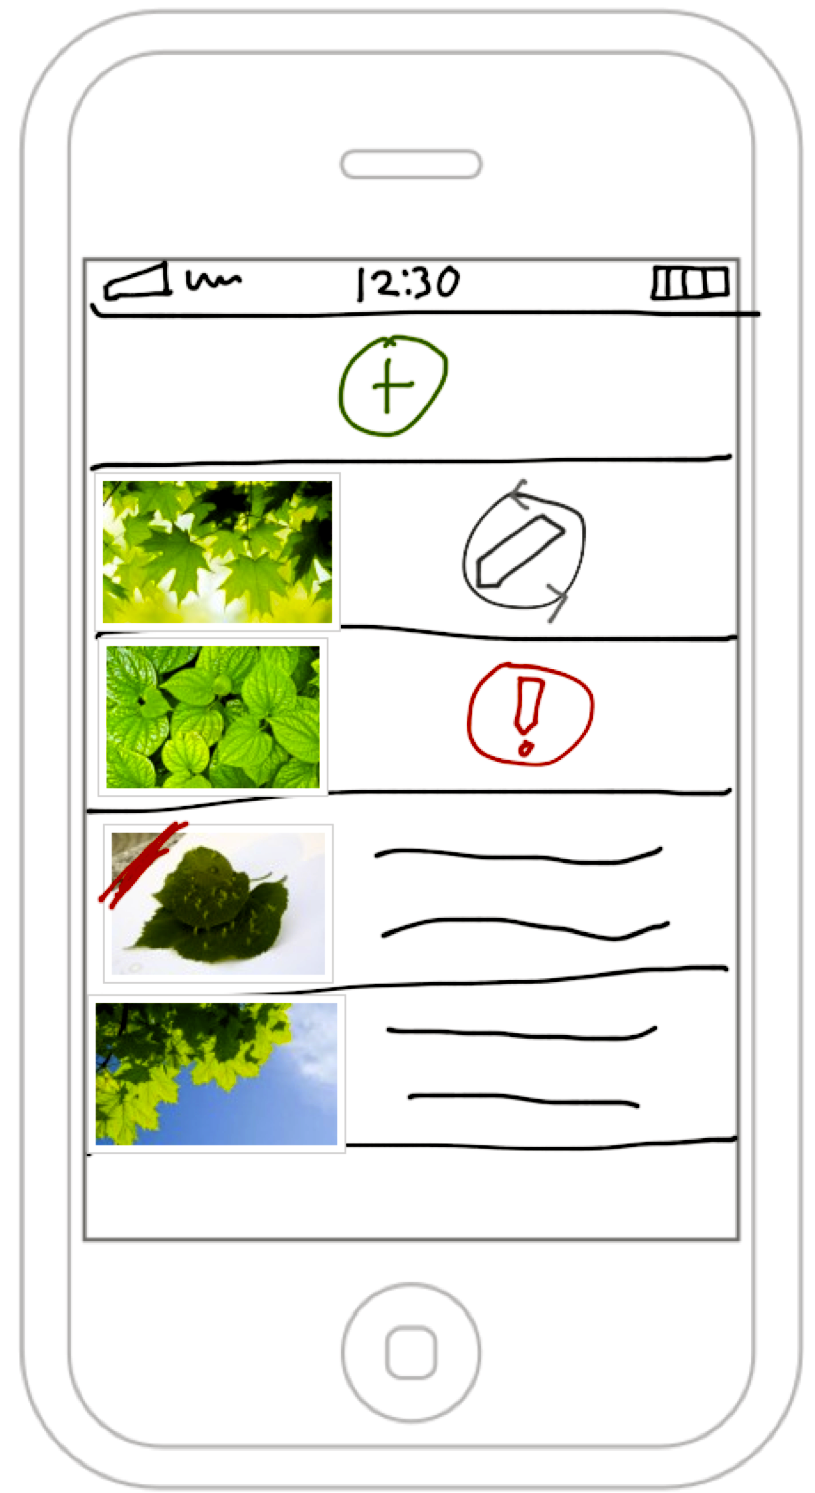
\includegraphics[width=0.19\linewidth]{images/BeLeaf3.png}
	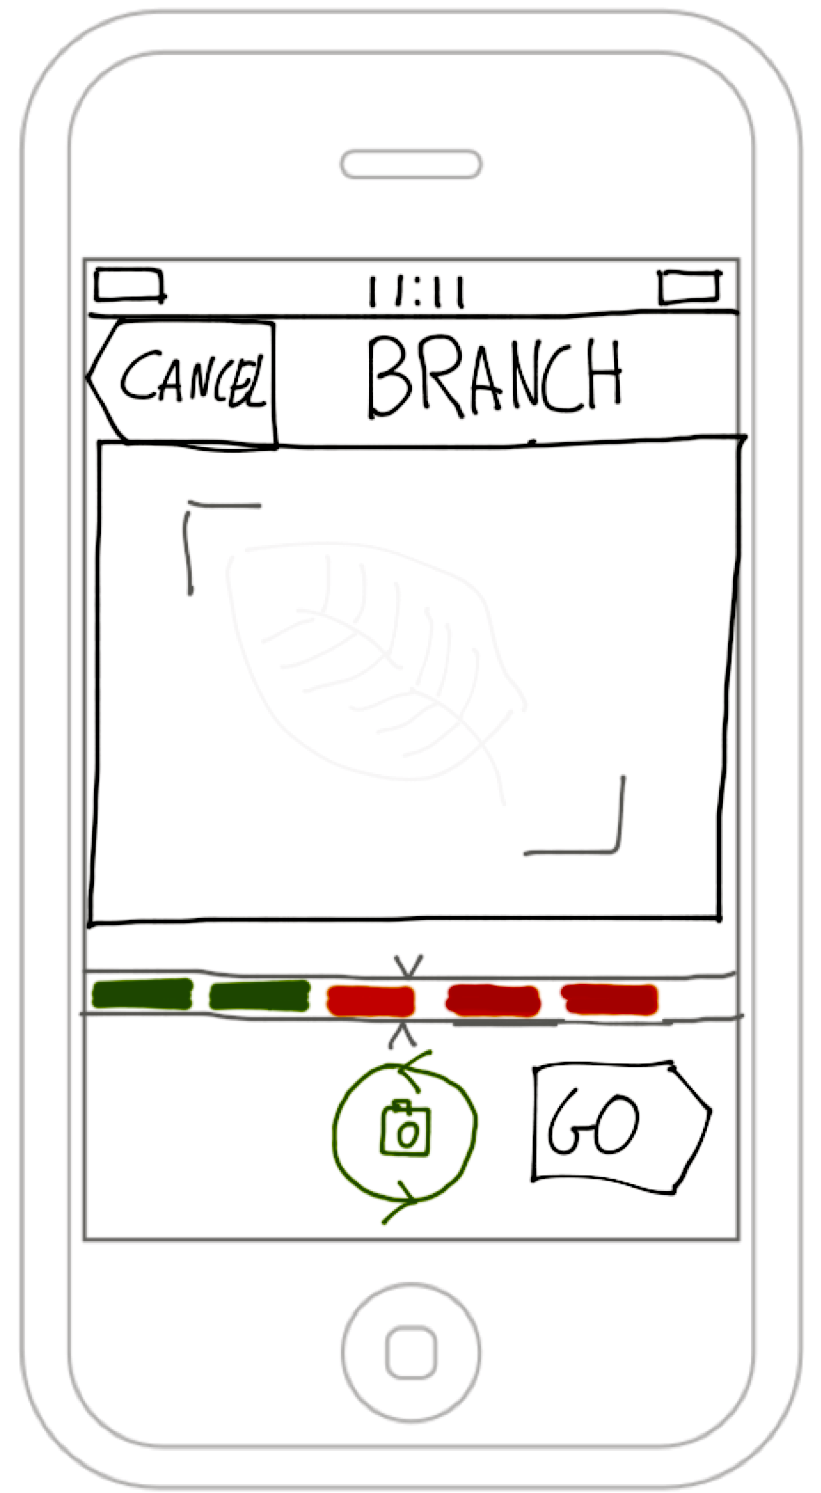
\includegraphics[width=0.19\linewidth]{images/BeLeaf2.png}
	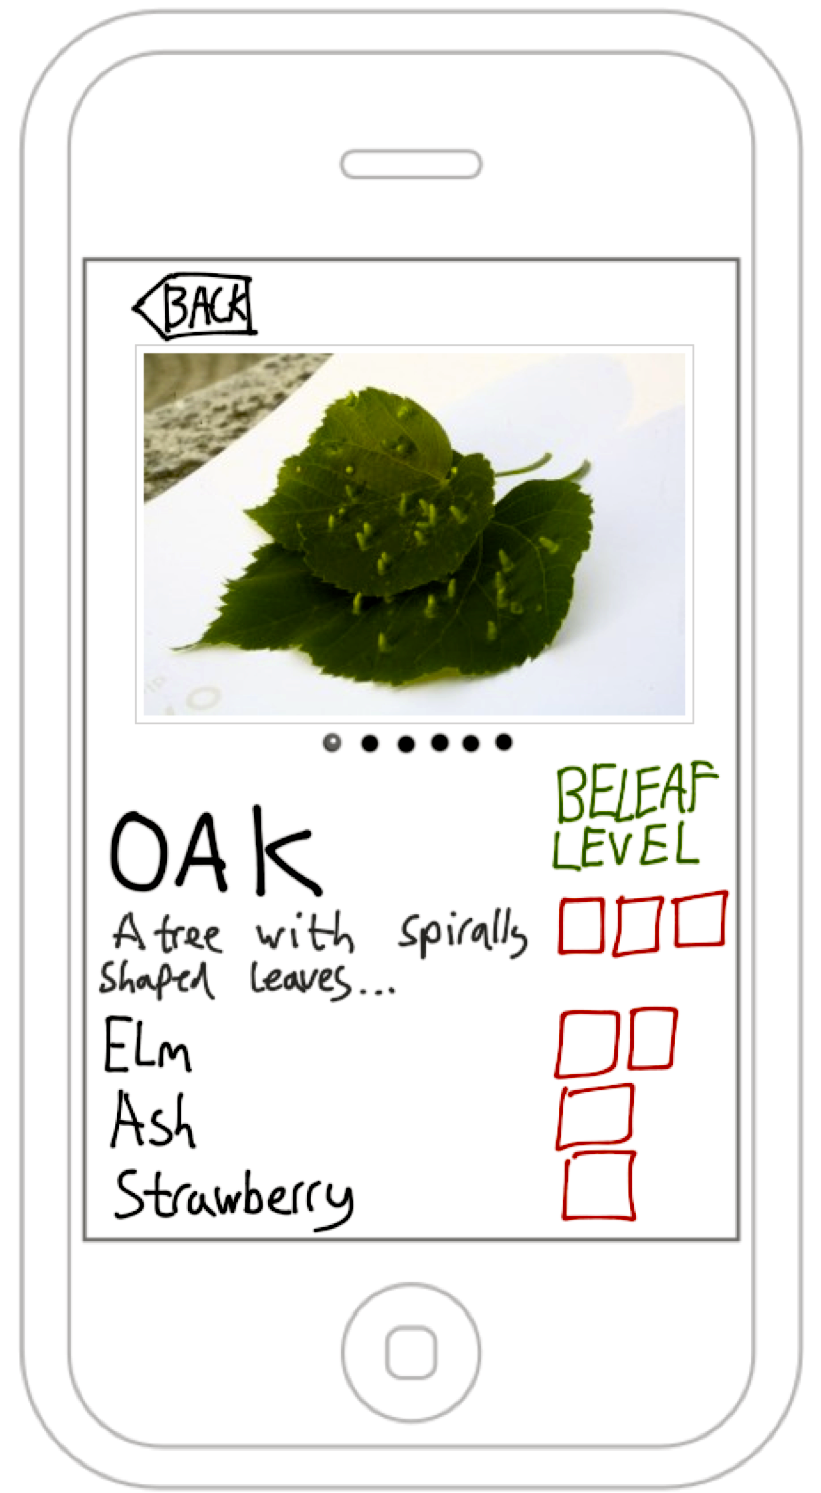
\includegraphics[width=0.19\linewidth]{images/BeLeaf4.png}\\
	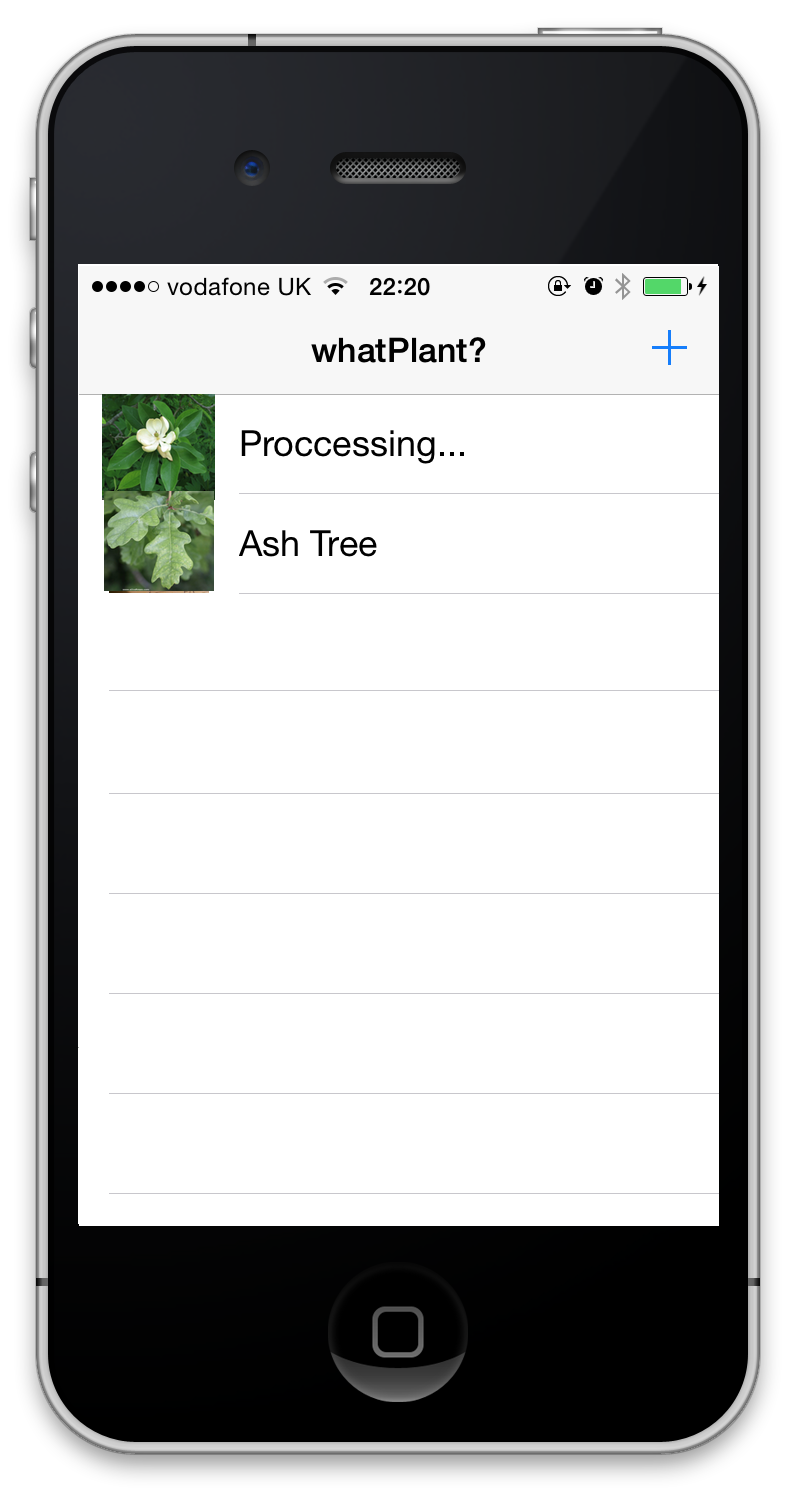
\includegraphics[width=0.19\linewidth]{images/prototypeScreenShot1.png}
	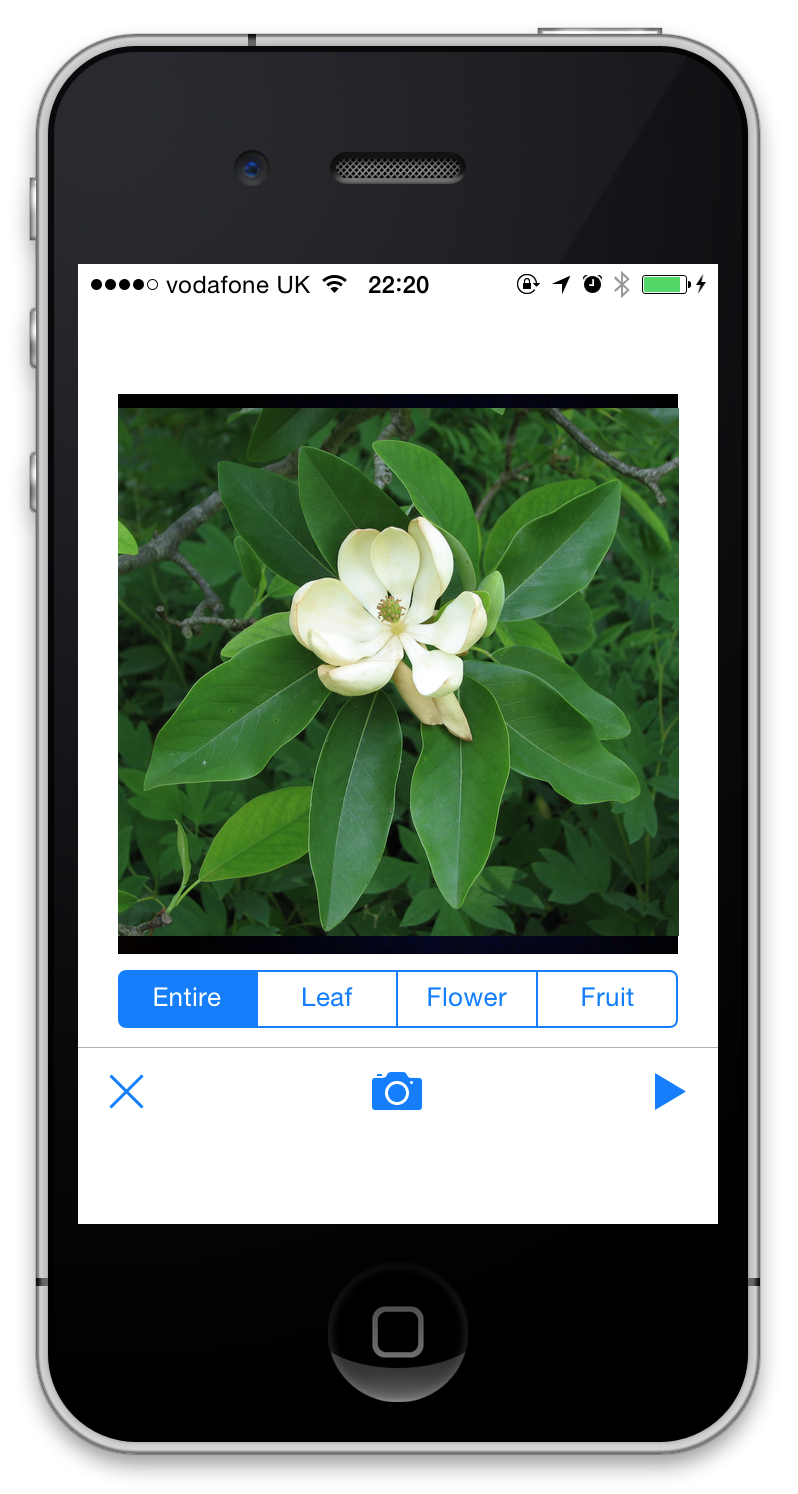
\includegraphics[width=0.19\linewidth]{images/prototypeScreenShot2.png}
	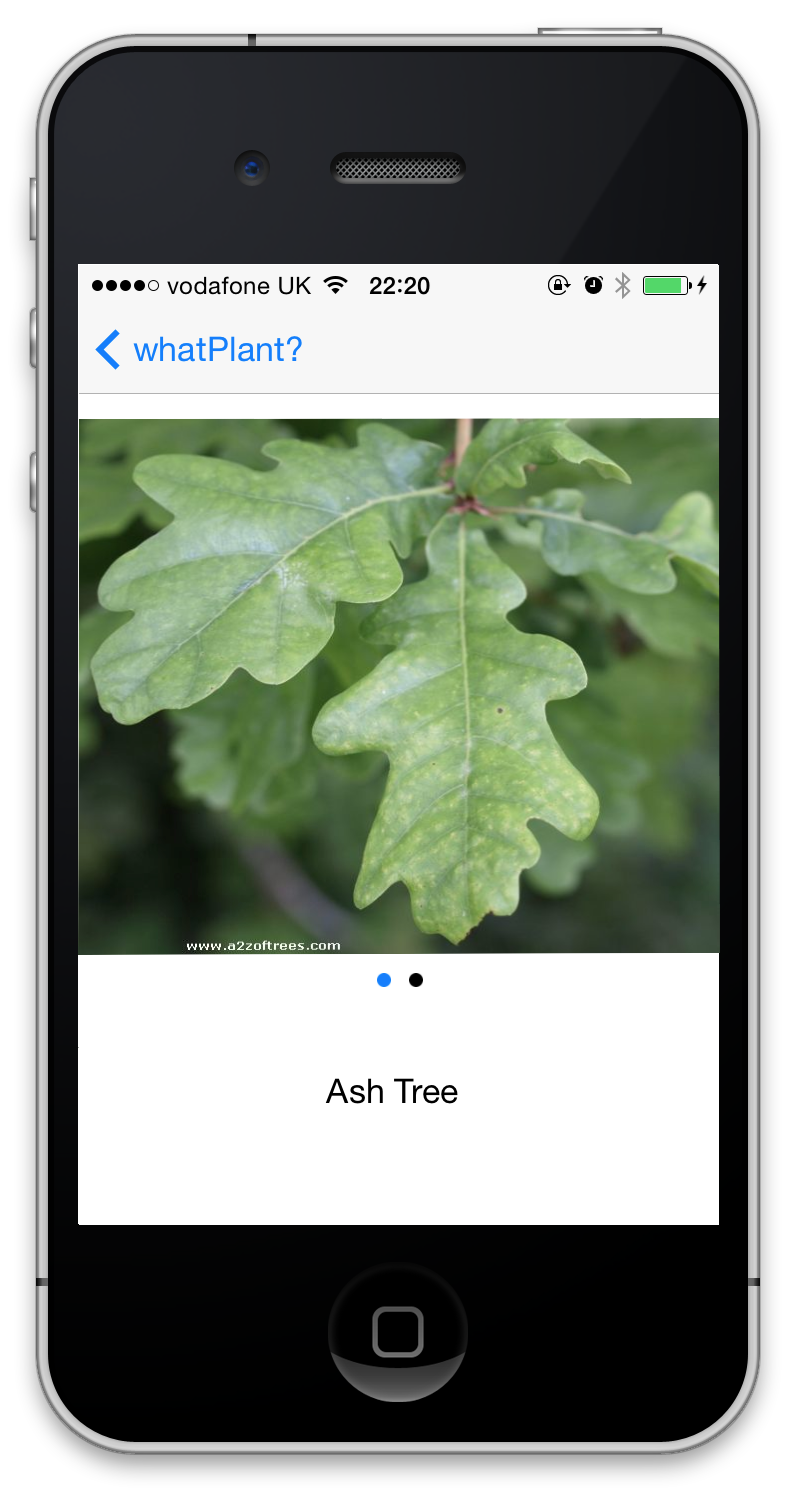
\includegraphics[width=0.19\linewidth]{images/prototypeScreenShot3.png}\\
	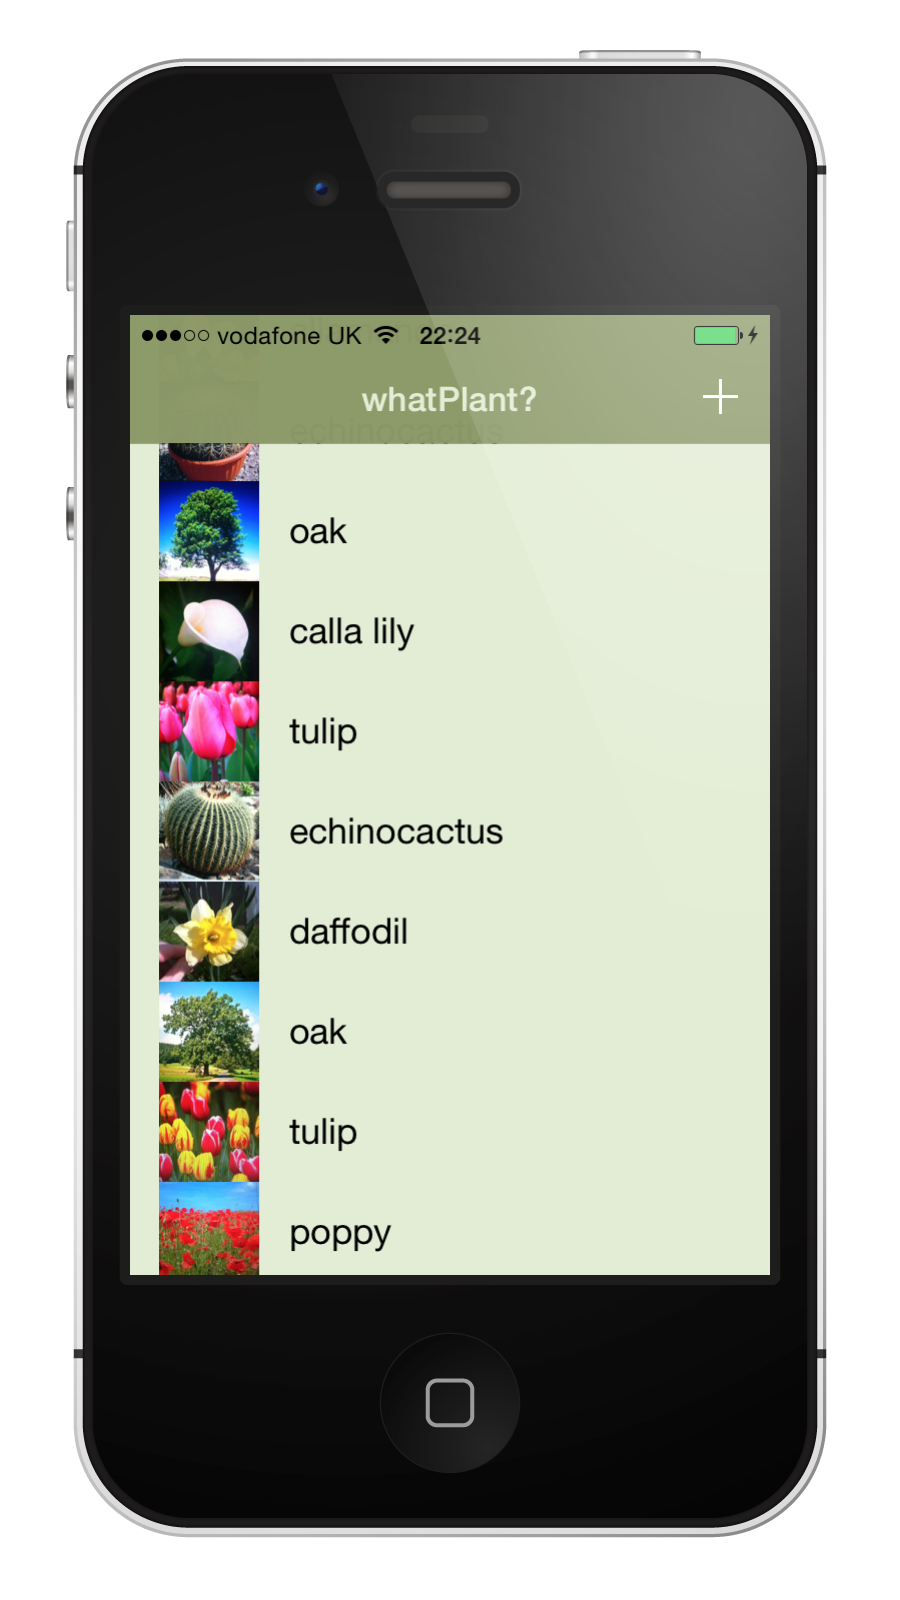
\includegraphics[width=0.22\linewidth]{images/release_1.png}
	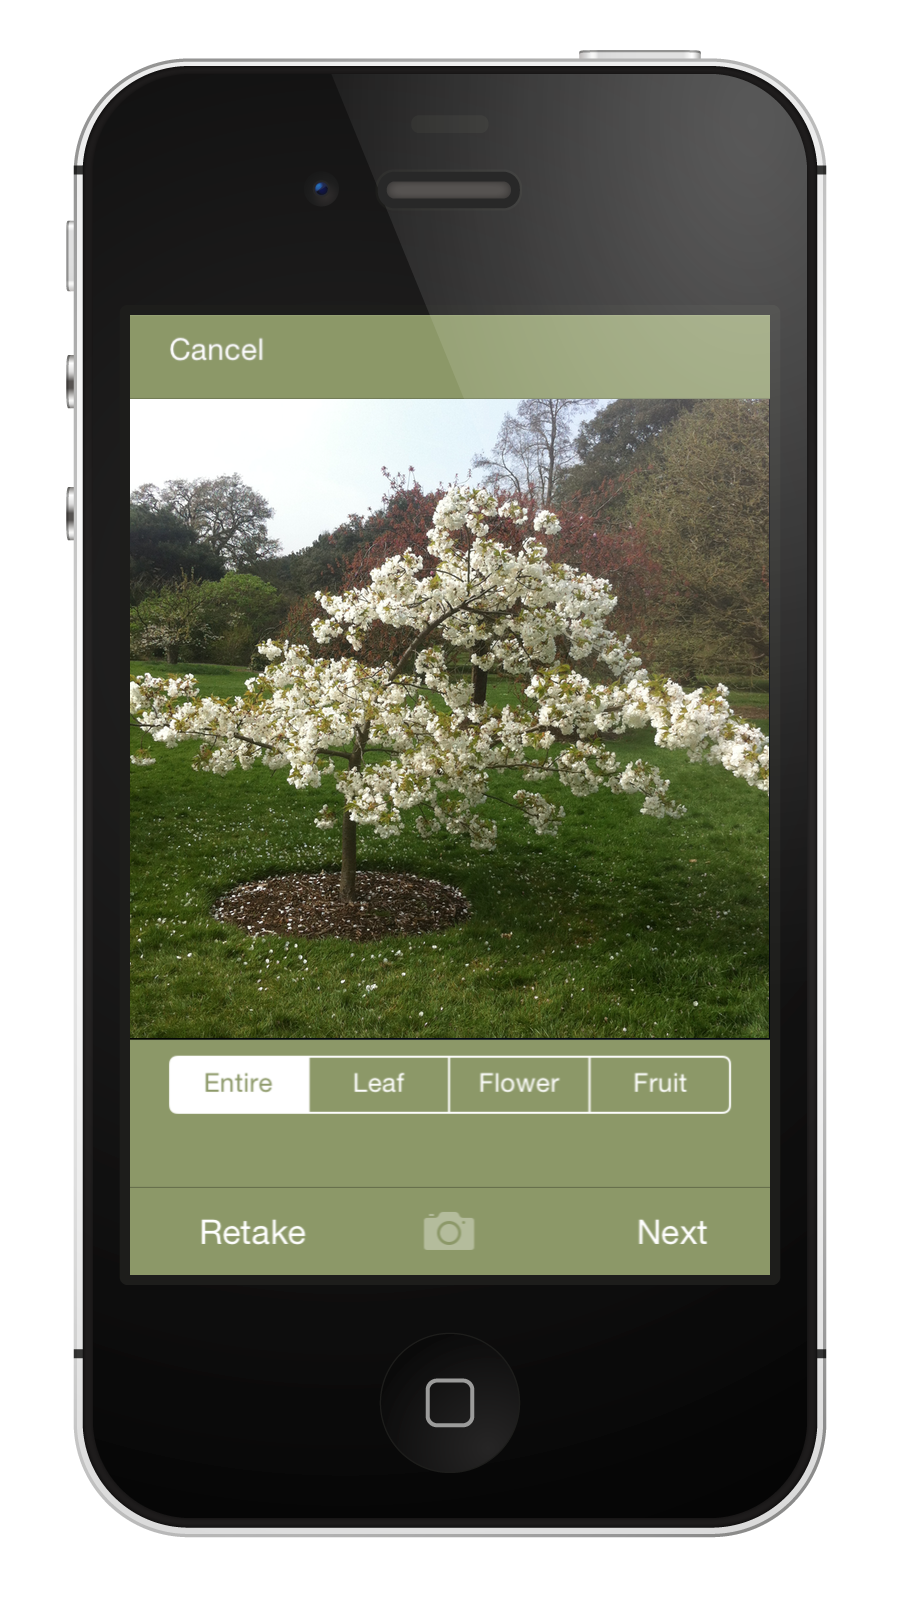
\includegraphics[width=0.22\linewidth]{images/release_2.png}
	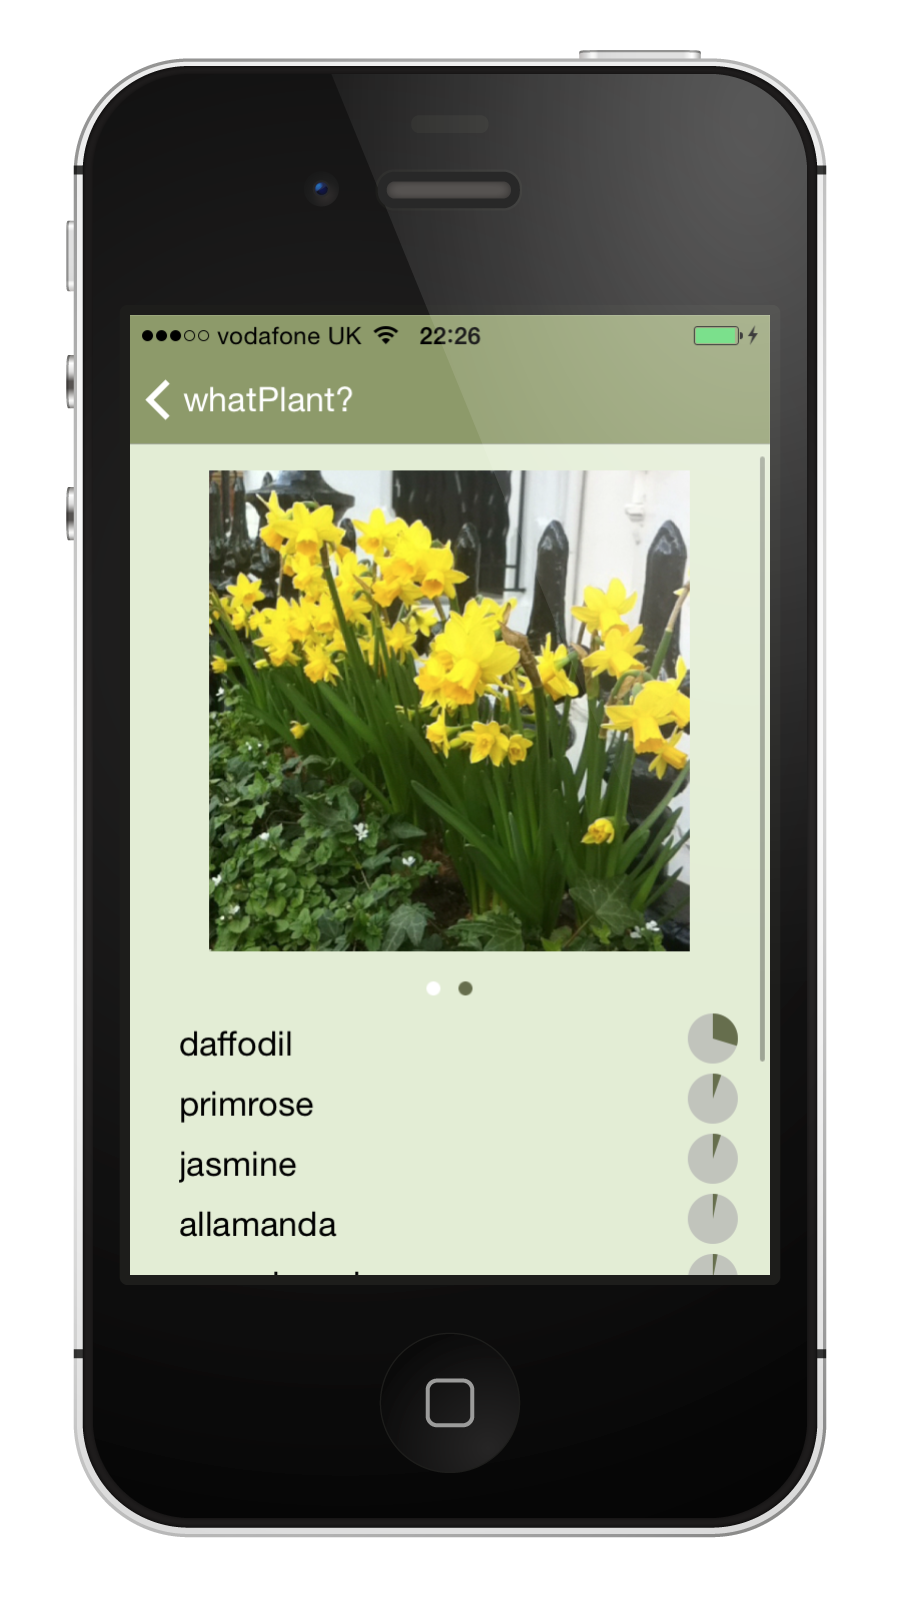
\includegraphics[width=0.22\linewidth]{images/release_3.png}

	\caption{Evolution of the App}
\end{figure}

\clearpage
\section{Methodology}

\subsection{Division Of Work}

We balanced the existing experience and skill set of each team member with their desired learning outcomes in order to best allocate resources and ensure timely delivery of each component of the specification. Due to his prior experience in software project management, Gerard Haughian was nominated as Group Leader and Scrum Master and accepted responsibility for Code Integration and Release Management.
\\
\\
The table below shows the initial allocation of individuals to areas:
\\

\begin{tabular}{ c c c c c c }
  & Leader & Doc Editor & Servers & Frontend & Machine Learning \\
  \hline
  Alexandre Dalyac & - & - & - & - & X \\
  Ashley Cutmore & - & - & - & X & - \\
  Gerard Haughian & X & - & - & - & X \\
  John McCormac& - & - & - & - & X \\
  Simon Leigh & - & X & X & - & - \\
  Stewart Douglas& - & - & X & - & - \\
\end{tabular}


\subsection{Agile Development}

The project management methodology of choice for this project was Agile software development with Scrum. Some group members have previous industry experience using Scrum and recognise the key benefits of using it and its popularity; often being the methodology of choice in the industry. Agile was favoured over other methodologies such as Waterfall due to the ability to incrementally produce a stable working product at the end of each sprint. This is beneficial as having something tangible to demo to stakeholders enabled the team to implement any feedback straight back into the product, rapidly respond to issues, and incrementally improve upon the product. We aimed to maximise code coverage by unit testing and using a sophisticated release management strategy that automated the majority of our unit and integration testing. This is explained in greater detail in section 5.4. 

\subsubsection {Anatomy of the Sprints}

The sprints were two weeks in duration. This length was favoured due to the complexity of the system and the number of components that needed to be developed. We also recognised that other academic commitments needed to be taken into account. The team completed three full sprints and one half sized sprint. 

\paragraph {Backlog}
The backlog was central to the project. The requirements were written up as user stories with associated acceptance tests. The backlog was updated before each sprint and frozen during sprints. It was contained within the project management tool VersionOne \cite{versionone}. This tool enabled sprint planning and progress tracking of the project over time.

Each user story was assigned a high-level estimate of the number of hours required to complete that story. We used buckets of 1, 2, 4, and 8 hours as the scale of choice for these estimates. The backlog was prioritised in order of importance of that feature making it into the final product.

\paragraph {Scrum Board}
VersionOne offered the necessary functionality to act as our online scrum board. Having one piece of software manage as many aspects of our project as possible was desired over using multiple applications. Having a central application ensured that we had accurate and up to date information on the progress of our project and the tasks each user was responsible for.

\paragraph {Daily Scrum}

During weekdays the team met at a designated time for daily scrums. These where between 5-10 minutes in duration and run by our Scrum Master, Gerard Haughian. Traditionally all members of the team would be physically present for this stand-up however if a team member was working remotely they would use Google Hangout to join the scrum.

\paragraph {Sprint Procedures}
Each sprint consisted of five stages:

\begin{itemize}
\item \textbf{Backlog Review:} Prioritise the backlog and select user stories that will form the sprint backlog. Add selected user stories to a new sprint on VersionOne.
\item \textbf{Estimations and Committals:} Prioritise the sprint backlog and assign estimations to the user stories. 
\item \textbf{Tasking Up:} Break down user stories into tasks and put those tasks on VersionOne assigning team members to work on them.
\item \textbf{Product Demo:} At the end of the sprint, demo the product to Mr. Kelly and Dr. Knottenbelt. 
\item \textbf{Retrospective:} As sprints were completed, we discussed what went well and identified areas of improvement for the next sprint. We quickly reviewed overall progress on the product backlog to ensure we where still on schedule to complete the project.

\end{itemize}


\subsection{Source Control}

We used git as our version control software of choice for a number of reasons: decentralised local actions that are extremely fast; almost everything committed is recoverable; cheap and easy branching encourages frequent use. Additionally, the release management strategy below highlights ways in which we attempt to alleviate one issue with git's decentralised system which could potentially lead to state in which there is no sense of a “latest” version of our code base. Git integrates well with GitLab which all members of the team have experience with. GitLab also enables setting up web hooks which we can utilise to trigger automated unit tests.

\subsection {Release Management}

A simple, well defined release management process was put into place that ensured we always maintained a stable, well tested and structured version of our code base. This guaranteed we always had a deployable product from early in the project and that development work completed during sprints did not affect our stable code base.

We had tiered release management strategy which consists of having three git branches, namely: DEV, QA and Master. When a team member began working on a task, they first checkout the DEV branch, then create a new branch from DEV named appropriately for the task they are working on. As each developer worked on completing a task, they could check code in and out of their task branch without affecting the main DEV branch. Once tasks were completed the code was merged and pushed into DEV, triggering automated unit tests.

This approach encouraged any new code checked into the DEV branch to have appropriate unit tests associated with it. This strategy assisted in detecting issues early and ensured all components of the system remained in a compatible state. Once all tasks required for a sprint where completed, the release manager pushed and merged all changes into the QA branch for Unit, System and Integration testing. At the end of each sprint, all new code was pushed and merged with the Master branch by the release manager. The Master branch always reflected a stable, well tested and incremental prototype of our system. 

Both the QA and Master branches where protected so that only the release manager could push code to those branches. It is expected that a few days prior to a sprint’s due date, all code is checked into QA for adequate testing before the release date. 

\begin{figure}[htb!]
	\centering
	%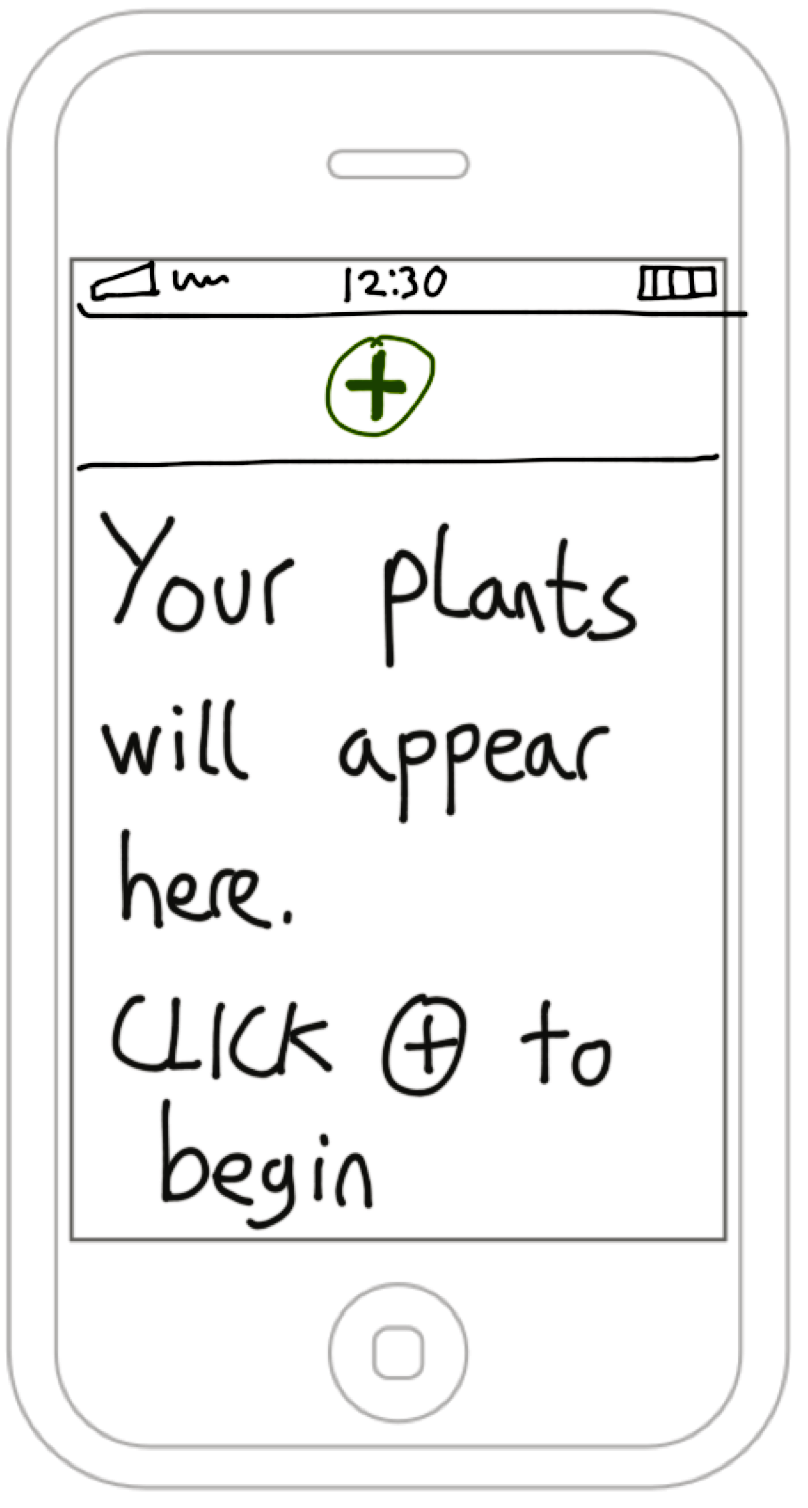
\includegraphics[width=0.22\linewidth]{BeLeaf1.png}
	%	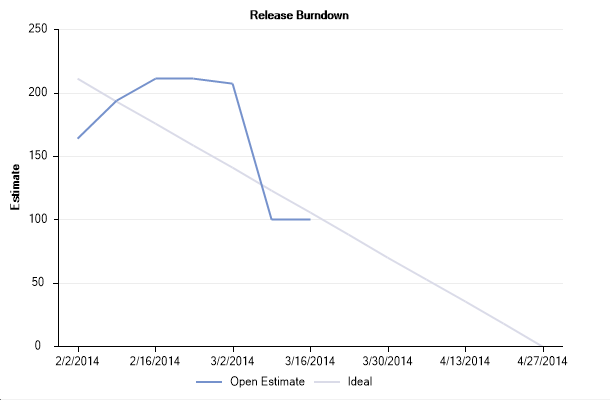
\includegraphics[width=0.50\linewidth]{images/release_burndown.png}
	\caption{Project Velocity Tracking}
	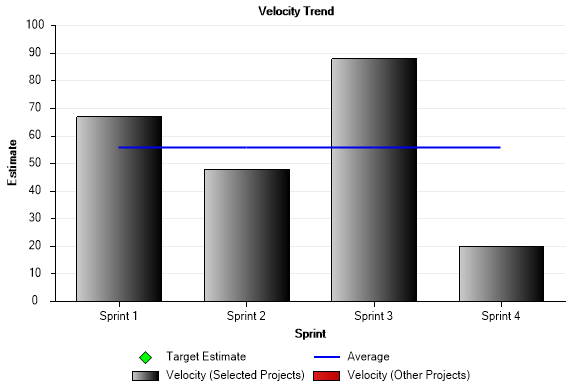
\includegraphics[width=0.80\linewidth]{images/VelocityTrend.png}
	\caption{Git Commit Statistics}
		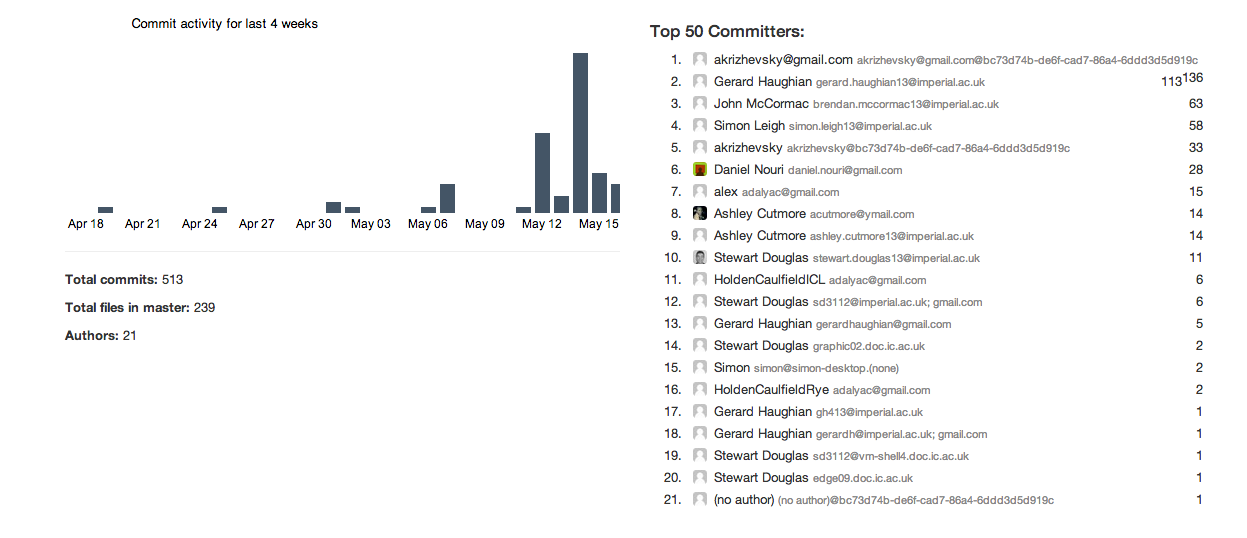
\includegraphics[width=0.80\linewidth]{images/GitCommits.png}

\end{figure}
\clearpage

\subsection{Testing}

The combination of several distinct pieces of software and multiple languages necessitated various tools for unit testing. A Continuous Integration server was built which automated unit testing after every check-in to our DEV branch. Tests were triggered at the end of each sprint when code was checked in to our QA branch, ensuring the integrity of our code base was maintained. Emails were despatched by the Continuous Integration server to notify group members of the results of these tests. Our integration and system testing involved using our prototype and verifying that a complete roundtrip classification was successful. Each subsection that follows highlights in detail the unit testing strategy employed for each component of the system. 


\subsubsection{iOS 7 Application}

The iOS application is written in Objective-C and makes use of Apple's range of frameworks for accessing hardware features on the iPhone (including camera and GPS) and the drawing of basic UI elements (buttons, images, animations). Xcode (Apple's IDE) is the main workhorse for developing the iOS application and comes with Apple's unit testing framework (xctest) built in.

Taking an initial Black-Box approach and writing tests for core classes before beginning to implement any functionality helped define exactly what each class was responsible for and how it would expose its functionality. As development of the classes proceeded a more White-Box approach was adopted. For example the core server interaction class has private methods for processing the server's JSON response, in Objective-C this could be exposed and tested with a variety of response data in isolation. This mix of the two approaches is described as a Grey-Box approach.

Unit tests should be both quick to execute and isolated of dependencies, to encourage frequent use and increase confidence that test failures point to a specific issue. To remove the delay and add isolation to the networking code the OHHTTPStubs library was used to `catch' calls made to the underlying Network API and redirected to a simple stub of the API that could return a range of HTTP responses instantly. Code coverage statistics were produced in Xcode by simply passing the appropriate flag to the built-in compiler, LLVM. Cover Story, an open source program, provides the ability to analyse and generate reports from the coverage files. Unfortunately branch coverage statistics are not produced. There are currently 37 unit tests and take $\sim0.3$seconds to run.

\begin{table}[h]
   \centering
    \begin{tabular}{|l|cc|}
    \hline
    Module & Statement Coverage & Branch Coverage \\ \hline
    Database & 77.6\% - 111/143 & na     \\
    FileSystem & 98.3 \% - 59/60 & na \\
    Networking & 85.2\% - 253/297 & na \\
    Image Capture & 86.7\% - 91/105 & na\\
    \hline
    Total Coverage & 84.8\% - 514/605 &  na \\      
    \hline
    \end{tabular}
    \caption {Code Coverage for iOS 7 application}
\end{table}

\clearpage
\subsubsection{Servers}

%The iOS application communicates with the Request server: an HTTP server running on the node.js platform and making use of the Express framework. The database used is MongoDB. The HTTP server exposes a RESTful interface \cite{ibm_restful} that provides the HTTP GET and POST methods in order to enable querying of our database and uploading of new images. 

%The Request server communicates with the Worker server. The Worker server makes use of the same technologies as the Request server and exposes a POST method to the Request server in order to allow transmission of uploaded images and accompanying metadata.

%Both servers are programmed in Javascript. The asynchronous nature of the functions presented some challenges when considering how best to unit test the code: the POST and GET methods require HTTP request and response objects to be passed into them. This necessitated the use of a test framework that provided the ability to construct the stubs necessary to simulate interaction with outside components.

A Grey-Box testing approach was used, given that multiple libraries were used for which we did not have visibility of all internal structure. Partition testing was used to select and test boundary cases and try to ensure effective, high quality unit tests.

Mocha \cite{mocha} was selected as the unit testing framework for the Servers, as it enabled straightforward testing of our asynchronous logic and the necessary integration with node.js, Express and MongoDB. 
Istanbul \cite{istanbul} was selected as the code coverage tool for our server-side Javascript. It has integration with Mocha (allowing tests to be run and coverage to be computed in one operation), tracks statement, branch, and function coverage and is able to produce easily parsed coverage outputs in XML, JSON or HTML. 

The combination of Istanbul and Mocha enabled straightforward creation and automation of our unit tests for the Servers.

%The reduced branch coverage for the POST and GET routes of the Request server are due to the difficulty in simulating particular database errors (such as a working database connection but an error when reading from a collection). These error types are to be handled in code branches, but it has not yet proven possible to produce a stub which can simulate the error.

\begin{table}[h]
   \centering
    \begin{tabular}{|l|cc|}
    \hline
    Module                 & Statement Coverage  & Branch Coverage \\ \hline
    Configuration Parsing  & ~   100\% - 52/52   & ~100\% - 22/22     \\
    POST and GET Routes    & ~   81\%  - 102/126   & ~77\%  - 26/34      \\
    Server Instantiation   & ~   88\%  - 46/52   & ~75\%  - 9/12     \\
    \hline
    Total Coverage         &     86\%  - 200/230 & 87\%   - 57/68	\\      
    \hline
    \end{tabular}
    \caption {Code Coverage for Request Server}
\end{table}

\begin{table}[h]
   \centering
    \begin{tabular}{|l|cc|}
    \hline
    Module                & Statement Coverage & Branch Coverage \\ \hline
    Configuration Parsing & ~   100\% - 52/52  & ~100\% - 22/22     \\
    Routes                & ~   88\% - 44/50   &  ~62\%  - 5/8      \\
    Server Instantiation  & ~   90\% - 52/58   &  ~86\%  - 12/14      \\
    Update Poll           & ~   88\% - 95/108   &  ~82\%  - 31/38      \\
    \hline
    Total Coverage        &     91\% - 243/268     & 85\%   - 70/82  \\      
    \hline
    \end{tabular}
    \caption {Code Coverage for Worker Server}
\end{table}

\clearpage
\subsubsection{Plant Classification}

Our plant classification framework uses a combination of CUDA C\verb!++! and python. The CUDA elements of Alex Krizhevsky's CUDA convnet library (as modified by Daniel Nouri to include dropout) have required no modification and so have not been tested. The modules which we have edited have all been written in python; hence we use a combination of the python unittest and coverage modules. We use a grey-box testing approach, ensuring a high code coverage of the individual units, while also ensuring all of the key specification criteria are met. Many of the test cases used partition testing to try and catch real world `edge cases'.

In the early stages of development, many very small one off scripts were written. These scripts do not form an integral part of our classification system and so have not been included under our test coverage framework. To properly test the infrastructure requires both the appropriate MongoDB server to be running, and a GPU to test our neural network run scripts.

\begin{table}[h]
   \centering
    \begin{tabular}{|l|cc|}
    \hline
    Module                                & Statement Coverage  & Branch Coverage \\ \hline
    Image Manipulation and Batching       & 83\% - 163/196      & 81\% - 47/58    \\
    Network Data Providers                & 96\% - 48/50       & 80\% - 8/10    \\
    Component Classification (run script) & 89\% - 143/161      & 73\% - 32/44    \\
    Classification Post Processing        & 83\% - 74/89        & 77\% - 23/30    \\
    Component Tagging                     & 78\% - 109/140      & 91\% - 29/32    \\
    Database Querying                     & 93\% - 51/55        & 79\% - 11/14    \\ \hline
    Total Coverage                        & 85\% - 588/691      & 78\% - 146/188           \\ \hline
    \end{tabular}
    \caption {Code Coverage for Plant Classification}
\end{table}

\subsubsection{Overall Coverage}

The overall coverage is given by taking the arithmetic mean across the sections.

\begin{table}[h]
   \centering
    \begin{tabular}{|l|cc|}
    \hline
    Module                                & Statement Coverage  & Branch Coverage \\ \hline
    iOS 7 Application                       & 85\% - 514/605    & na		  \\
    Request Server                          & 86\% - 200/230   & 87\%	- 57/68	\\
    Worker Server                           & 91\% - 243/268    & 85\%  - 70/82  \\
    Plant Classification                    & 85\% - 588/691    & 78\%	- 146/188	\\ \hline
    Total Coverage                          & 87\% - 1545/1794  & 83\%	- 273/338	\\ \hline
    \end{tabular}
    \caption {Overall Code Coverage}
\end{table}

\clearpage

\section{Implementation}

%What were the intellectual and/or technical problems that had to be solved? What techniques did you consider using for solving the problem? Which did you choose and why?
Below, we list the challenges involved in the implementation of each area of the project and the solutions we developed to overcome them.

\subsection{iOS 7 Application}
\begin{description}

\item [Challenge:] \textit{Concurrency}\\\\
To ensure a positive user experience, multi-threading was required to keep the UI interactive and responsive while other tasks were performed in the background. Multi-threaded code can be beautifully simple when threads can lock access to shared data or are given immutable data, however this is not always possible when users are involved. For example: A `specimen' object is needed by the network thread to generate the appropriate network requests to send to the server and possibly make updates. What should happen if the user decides to `swipe-to-delete' that specimen from the table during the network task? To the user it would make little sense why this action might be blocked and even if every line of the network code was protected by an `if object still exists' guard it would still not be thread safe. To overcome this, when a user deletes a specimen it is only made invisible. It appears to have been deleted but still resides in memory, except it now has its `deleted' flag set. The actual deletion can be done at a safe, controlled time such as app start up or termination.\\


\item [Challenge:] \textit{App Store Submission}\\\\
The second main challenge was releasing the app on the App Store. It was a long and involved process requiring continual monitoring, discussions, and a number of non-code related tasks, such as designing a logo and brand. One particularly difficult element of our submission was the requirement for our whole infrastructure, from the server to the classifier, to be up and running for the duration: the submitted App could be tested at any time by Apple. This unfortunately led to a significant delay in training our neural network, as well as pending improvements for performance of both it and the Worker server.  We also set up a number of systems to alert us to any issues with the server, to ensure it continued working as expected. The benefit of this hiatus was that it proved that the full system could be up and running for an extended period of time, supplying classifications to outside users. Our application was approved before the submission of this report, and is now scheduled to go up on the App store.
\end{description}

\subsection{Servers}

The main considerations we faced in selecting the software stack for use in our servers were: scalability, stability, compatibility with our database, and ease of implementation.

Both servers are implemented using Node.js with the Express web application framework. MongoDB is our chosen database. Node.js is built on Google Chrome's JavaScript V8 runtime environment. It was selected since it is well supported and easy to develop in. It is highly scalable and easily implements asynchronous data calls making it well suited to our project \cite{nodejsabout}. MongoDB is a NoSQL document-orientated database which stores data in a compact JSON format known as Binary JSON. MongoDB interacts well with Node.js and the JSON format allows easy message passing with the rest of the stack.

\subsubsection{Request Server}

\begin{description}

\item [Challenge:] \textit{Concurrency and Scalability}\\\\
As an iOS application may well have a large number of concurrent users, we required a solution that would be able to support high simultaneous demand. Since our classification engine requires special hardware and must devote significant resources to classification, we isolate the Request server on another machine so that it may maintain significant, dedicated resources to accept and respond to HTTP requests received from the iOS application.

\hspace{5 mm} Node.js was selected as the environment as it has been proven to cope with many concurrent connections (in fact, up to 1m concurrent connections have been demonstrated \cite{nodeload}) and allows the use of full stack JSON along with MongoDB. 

\hspace{5 mm} MongoDB was chosen as our database solution as the document model fits well with the data that we must store. Additionally, the ability to shard MongoDB across multiple instances gave us the confidence that we would be able to easily scale out our database if demand proved sufficient.

\hspace{5 mm} RESTful HTTP interaction was selected as the means by which the Request Server, Worker Server and App would communicate. We chose this mature and portable standard to ensure that we would be easily able to introduce new platforms, and to enable the production of an open API, should it be desirable in future. \\

\item [Challenge:] \textit{Grouping Multiple Images for Classification}\\\\
As we allow the user to take multiple images of a single specimen, we must aggregate these segment images into a group, for which we can track the classification state. Apple impose significant restrictions on the ability of iOS applications to uniquely identify hardware or application users. Thus we accomplish the aggregation of data and session tracking by having the Request Server creating a new group document in the MongoDB database when the first image of a new set is received from the iOS application. The initial HTTP response that is sent to the iOS application then contains the unique `GroupID'. Further image submissions for the same specimen then have the GroupID embedded in the HTTP POST request made by the iOS application.

\hspace{5 mm} MongoDB, as a document based NoSQL database, is an ideal fit for our needs, as we embed the multiple individual segment `ObjectIDs' that represent each image in one `super' document representing the group of images for a single specimen. Queries and updates can then be made to all documents belonging to a group, or to individual documents within that group. We may then store the ultimate classification against the `Group' document.

\hspace{5 mm} Once the user confirms via the iOS application that they have finished uploading images of a specimen, an HTTP PUT request is sent to the Request Server containing the unique ID of the `Group' which is now complete. The appropriate document is then updated in the database, so that the Worker server may then combine the individual classifications for each image into one classification for the whole group.

%Each segment document contains the following information in the JSON format. We store the image metadata to enable further analysis, and provide the means for us to enhance features in future (such as tracking invasive species using the longitude and latitude data provided by iOS).

%\begin{verbatim}
%{ _id,
%  filepath,
%  group_id,
%  submission_state,
%  submission_time,
%  image_metadata : { date , latitude, longitude },
%  image_segment }

%\end{verbatim}

%As each segment image is uploaded by the user, the information is extracted and added to the database. Once the call to the database returns with a unique segment identifier, an HTTP POST request is constructed by the Request Server which despatches the binary image data and relevant database document IDs to the Worker Server. In this way, we completely decouple the functions of the Request and Worker Server and allow for them to be on remote machines, and require only an HTTP/TCP session to be established between them.


\end{description}

\subsubsection{Worker Server}
\begin{description}
\item [Challenge:] \textit{Receipt of Images}\\\\
The Worker Server oversees the storage of user images and the querying of the neural net. It listens for HTTP POST requests from the Request Server, and on receipt of a new image stores the image in a directory created specifically for that image's group. At the same time as it is listening for new images to be sent to it, the Worker Server polls the MongoDB database for images which need to be sent to the neural network for classification. If such an image is found then a link to the images location is passed to the neural network, which genertes a .pickle data file for classification. Some of these actions need to be executed synchronously: a new group folder must be generated and a new image saved into this folder prior to passing the image to the neural net. Like the Request server it makes extensive use of \textit{formidable} for extracting form information. It also makes use of of the \textit{mkdirp} library to synchronously create a new directory. When a new image has been received the Worker server will update the MongoDB database, and the image's relevant entries will be updated to reflect the fact that it is now ready for classification. \\

\item [Challenge:] \textit{Synchronous Execution}\\\\
As noted in the previous point, many of the Worker Server tasks must be completed synchronously. For example, we should not attempt to pass multiple images through the net at the same time. This is complicated by the fact that Node.js is asynchronous by default, and so we needed to rely on third-party libraries to make sure certain sections of the code blocked until completion. Initially we used the \textit{async} library, but this depended on using timeouts which led to longer response times. For our final implementation we use JavaScript `promises', which allow us to write synchronous code is a concise and readable way. The \textit{Q} library was chosen because it was well documented. 
\end{description}
\subsection{Plant Classification}

\begin{description}

\item [Challenge:] \textit{Computer Vision}\\\\
There are three considerable computer vision problems: number and complexity of features, image segmentation, and the need for translation invariance. Specifying at the pixel level what features define each class would require expert botanical knowledge of each species and enormous effort spent hard-coding detectors for each feature. Secondly, in order to recognise a plant in an image, the target needs to be segmented from the image. If the plant is in the wild, conventional segmentation approaches based on edge and corner detection are of little use; hence why LeafSnap requires the target to be placed on a white background. Thirdly, the need for translation invariance, as an object remains the same regardless of where it is located within an image.

\hspace{5 mm} We opted for a Deep Learning approach to classification, because it can automatically learn features. It learns features that work best on a training set, so with wildlife training images, features are learned that deal with segmentation. We specifically chose a Convolutional Neural Network (CNN) implementation, the architecture of which is inspired by that of the human visual cortex, and is specifically built to replicate feature detection across all dimensions. This is known to deal efficiently with dimension hopping by achieving translation invariance. Although there are many alternative methodologies (SIFT, Random Forests, and SVMs to name just a few), the record breaking performance of Alex Krishevsky's cuda-convnet \cite{cudaconv_2012} project on the same data source we had available \cite{imagenet} and with a comparable number of classes, made it an ideal library upon which to base our classifier.\\

\item [Challenge:] \textit{Data Processing}\\\\
Deep learning itself is distinguished from other machine learning techniques by not simply learning the relative importance of features, but by learning the features themselves. The additional information needed for this raises the desired volume of training data. The PlantCLEF dataset which was originally intended to underlie training, provided a meagre average of 12 images per species; our data sourcing pursuits managed to bring this number up to 2,000 per species. The only significantly large labelled dataset was ImageNet. 

\hspace{5 mm} To ensure our neural network wasn’t burdened having to learn to recognise species for which we had a limited training subset. A Bucketing algorithim was created in order to bucket those images into a higher level in our taxonomy tree which we constructed using WordNet\cite{wordnet}. This meant we could decrease our neural network error rate while maximising our use of available training data. Outlined below is the pseudocode for the bucketing algorithm.\\

\begin{algorithmic}[1]
\Procedure{bucketing}{}
	\State $NumPlants \gets$ global hash table with aggregated count of unique plants
	\State $leafNodes \gets$ set containing all leaf nodes in the plant taxonomy tree
	\ForAll{$nodes \in leafNodes$}
		\Call{Update-Descendant-Count}{$nodes.PathToRoot$}
	\EndFor
	\ForAll{$nodes \in leafNodes$}
		\Call{Assign-Buckets}{$nodes.PathToRoot$}
	\EndFor
\EndProcedure 
\Statex
\end{algorithmic}

\begin{algorithmic}[1]
\Procedure{Update-Descendant-Count}{path}
	\State $count \gets 0$
	\ForAll{$nodes \in path$} 
		\State $count \gets count+NumPlants[node]$
		\State UPDATE Bucket = node, BucketSpecies = Species, Count += count 
		\State		FROM plants 
		\State		WHERE SynsetID = node
	\EndFor
\EndProcedure 
\Statex
\end{algorithmic}

\begin{algorithmic}[1]
\Procedure{Assign-Buckets}{path}
	\For{$i \gets 0 ... path.length$}
		\State $bucket \gets path[i]$
		\State $count \gets NumPlants[bucket]$
		\If{$count >= threshold$}
			\State UPDATE Bucket = $bucket$, BucketSpecies = species 
			\State		FROM plants 
			\State		WHERE SynsetID IN $path[0 ... i]$
			\State break
		\EndIf
	\EndFor
\EndProcedure 
\Statex
\end{algorithmic} 


Our final bucketing parameters for the network set a minimum threshold per class of 2,000 images, which resulted in total 1.2 million images, and 259 separate plant classes.

\hspace{5 mm} Our training images, originally in JPEG format were scaled (uniformly so as to preserve the aspect ratio) and cropped into square 256x256 3-channel images. These were then batched into groups of 128 and stored in python numpy arrays; this reduced preprocessing requirements making the CPU available for the more computationally intensive data augmentation stage (discussed below). The image size of 256 was chosen for a number of reasons: the cuda-convnet library was optimised for 256x256 images, we felt there was enough detail for plants of different species to be recognised at that resolution, and finally in the highly uncompressed numpy arrays, a larger image size would have used more space than our 2TB hard disk would allow.

\hspace{5 mm} Data augmentation was also an essential part of preventing overfitting on our neural networks; by using label-preserving transformations, such as extracting subpatches from images (in our case, 224x224 patches) taking horizontal reflections, and altering the intensities of the RGB channels with Principal Component Analysis. We used these techniques to increase the variation between successive training batches, and also take advantage the otherwise free CPU while the GPU was training the network weights.\\


\item [Challenge:] \textit{Network Architecture}\\\\
We experimented with two flavours of architecture.  The first was a single large network trained on the entire labelled dataset, the second was a combination of multiple smaller networks each trained to classify a specific plant component (Leaf, Flower, Fruit, or Entire).  We felt the multiple smaller network would have the advantage of learning a more specific set of features, as well as leveraging information provided to us from the user about the exact type of image being uploaded, which could help to improve accuracy. However two key potential drawbacks of smaller component networks were also apparent. Firstly, each component network would only have a small subset of the images which would work to counter performance gains of the more specific feature sets.  Secondly, on a single GPU system, the turnaround time for each user request would be much slower, as a new network would need to be loaded into memory for each component type submitted.


\begin{figure}[h!]
	\centering
	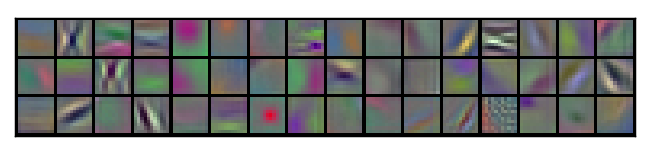
\includegraphics[width=0.80\linewidth]{filters.png}
	\caption{Filters learned by the plant recognisers first convolutional layer}
        \label{fig:ml_filters}
\end{figure}


\hspace{5 mm} The ImageNet data we had available, was tagged by species (such as Oak), but not by component type (Leaf, Flower, Fruit etc). We therefore trained a separate network on these separate component types (using PlantClef data \cite{plantclef}, which was tagged appropriately), and used that network to tag each of our 1.2 million images from ImageNet. The component network itself was based on the CIFAR training network \cite{cudaconv}, but modified to accept 256x256 resolution images.  We reserved 15\% of our component training data for accuracy testing, which achieved a 12\% top-1 error rate, giving us confidence to let the tagging proceed as planned.

\hspace{5 mm} We trained the Flower component network as an initial test, as it had the largest subset of images and hence we believed would exhibit the best performance.  However, after over a week of training, the best top-5 error rate achieved was 28\%, which was not significantly better than the performance of the single large net and had the drawbacks already discussed. Given that this was the best performance we were likely to achieve, we decided to use the single large network architecture for our production implementation.

\hspace{5 mm} The simpler, single large net was based heavily on Krishevsky's ImageNet architecture \cite{cudaconv_2012}. The network consisted of 5 convolutional layers (with max pooling and local response normalization), and 3 fully connected layers. The network use rectified linear unit neurons, which have been shown to significantly improve training times \cite{cudaconv_2012}.  The network was trained for 12 days on a single GeForce GTX 780, with 259 different plant classes. Each class has on average approximately 4,500 separate images. The top-5 error rate achieved for 102,400 test and cross-validation set cases was 29\%.  

\begin{figure}[h!]
	\centering
	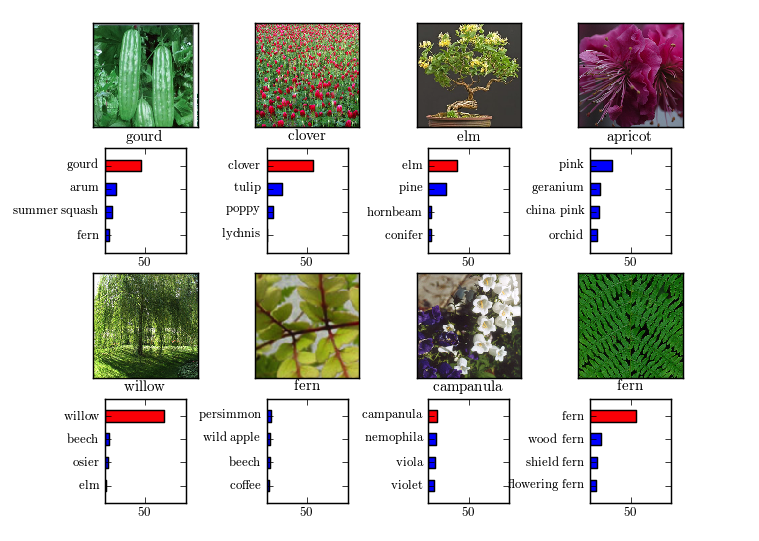
\includegraphics[width=1.0\linewidth]{preds.png}
	\caption{Some random predictions of previously unseen plant images}
        \label{fig:ml_preds}
\end{figure}

\section{Final Product}

\subsection{Product Evaluation}

%Description of the final product you have produced, i.e. your overall achievement.
%What have you implemented? Anything not implemented? What were the difficulties?
%Any difficulties you managed to overcome? Any results (this would apply more to
%investigative projects than to implementation projects)? Testing: how did you test
%it and what are the results? Evaluation: How good is your product, how well does
%it perform, how accurately does it satisfy the specification? 

We have succeeded in releasing an iOS App for recognising plant species in the wild. We have succeeded in developing a deep-learning convolutional neural network that can classify plants. Every task agreed, and highlighted in the Specification section as Essential have been achieved. We have in effect, delivered a product that meets the original specification. This includes creating the first ever App that automatically recognises diverse species of plants in the wild.

\subsection{Comparative Performance}

The performance of our app can be compared to its two competitors, LeafSnap and Google Goggles. Ours is the only one which can recognise plants in the wild. LeafSnap can only recognise leaves, and needs the leaf to be torn off and placed in front of a white background. Google Goggles aspires to recognise any class of object (e.g. painting, monument, plant, animal etc), but fails on plants. In fact, its ``overview and requirements'' page warns the reader that its performance is ``not so good'' with plants.\\

\begin{table}[h]
   \centering
    \begin{tabular}{|l|ccc|}
    \hline
    Image Set & Number of Images Tested & Top-5 Error & Top-1 Error \\ 
   \hline
    Test Batch & 88,320 & 29.0\% & 54.6\%      \\
    Cross-Validation Batch  & 14,080 & 29.4\% & 55.2\%      \\
    \hline
    Overall & 102,400 & 29.1\% & 54.7\%      \\     
    \hline
    \end{tabular}
    \caption {Overall Performance of our Neural Network}
\end{table}

\subsection{Further Development}
We have identified several areas where we feel we that optimisations are possible.\\

\begin{itemize}
  
 \item \textbf{Ensuring High Server Availability and Robust Error Checking}
 
Users of an iOS application have a justifiable expectation that the application works, regardless of the time of day. In our case, this means keeping our servers up and running 24 hours a day. This provides many challenges, but one in particular is the handling of error conditions occurring within our code. We cannot simply allow a server that experiences an error to gracefully exit and log the failure for later inspection. The server code should continue to run and receive and respond to the requests of other users, whilst logging the error.
We have tried to accomplish this by catching all errors and logging them, but there remains a danger that whilst the server code continues to run, it or the database may be left in an inconsistent state that may result in undefined behaviour.
We believe that a priority in further development would be the creation of monitoring scripts that monitor the health and consistency of items in the database and the results being produced by the Classification Engine and Request and Worker servers. These scripts would cleanse the database of old, unclassified jobs and remove any erroneous data, as well as monitoring the speed and viability of responses sent to the App.\\


\item \textbf{Enforcing Schema on a NoSQL Database to Prevent Inconsistent State}

Whilst the use of MongoDB provides us with great speed and scalability, the lack of an enforced schema means that is is incumbent upon the developer to ensure that all documents inserted or updated are consistent with their proposed data schema. We have been successful in this goal, but it has required significant collaborative effort.
A point for further development would be the production of schema configuration files, within which variables and constants could be contained and read in by each code component that made use of the database. In this manner we would enforce greater schema consistency across our code-base.\\


\item \textbf{App Responding to Server-Side Error Conditions}

The user-facing server protocol we devised during the early project meetings, though sufficient for our needs, did not included error handling. The App currently responds to errors by waiting for a set time period and retrying silently (without notifying the user). We could improve upon this by agreeing on both an error message the server could return on consistent classification failure (e.g image corruption) and a time-out period to stop retrying. The spinning classification processing icon could then turn into an exclamation mark and when `tapped' by the user, an error message displayed informing of the possible cause (network issues, image error). Finding the right balance for the time-out will require user research and prolonged software testing to ensure the time is long enough for the server to respond even when under pressure but short enough for the user to not become frustrated from lack of further information.

\end{itemize}

\subsection{Future Opportunities}

The commercial opportunities of WhatPlant are also of interest. A user spotting a pleasing plant in a park needs to identify its species in order to order the specimen in a shop. This places WhatPlant at a significant vantage point in the gardening consumer life cycle. The App could be augmented with hyperlinks to purchase the recognised plant specimen on partner e-commerce platforms and earn a commission on a per-click and per-purchase basis. We have already have many signups on our website, whatplant.github.io, which suggests a strong level of interest among the general public.

\hspace{5 mm} Another opportunity lies in the creation of citizen science initiatives for the control of invasive species. The GPS mapping capability of a smartphone could be coupled with the app's species detection to monitor ecosystems and flag new species.

\hspace{5 mm} The most attractive aspect of our project is its modularity: WhatPlant could be forked to produce WhatDog, WhatCat, WhatFish, WhatBird, WhatFabric, WhatDrink with relative ease, considering the data availabilities on ImageNet. The servers would require no modification, the machine learning would only require retraining, and the UI would only require minor adjustments such as a new logo.

\subsection{Project Evaluation}

Overall, we will certainly classify this project as a success. We all feel that we have learned a great deal about both the technical implementation of our chosen software, and how modern software development techniques are put into practice and the benefits they offer. The group worked very well as a team, all remaining dedicated to the project, putting in the extra hours and respecting each other's opinions. We are proud of what we have produced, and each of the group can attest that they contributed their fair share of work to the end result. 

\hspace{5 mm} Finally, we would like to thank our supervisors Dr William Knottenbelt and Mr Jack Kelly for their constant support and ineffable enthusiasm.

%In order to boost classification performance, WhatPlant could nurture a crowdsourcing community, with quality standards set by reputation points in a fashion similar to that of the stackexchange forums. Expert users could correct mistagged images and upload the image to contribute to the training database.

%WhatPlant could also be applied to mushroom picking, for which identification is crucial to safe consumption.



\clearpage

\begin{thebibliography}{1}

% Example: \bibitem{One}

\bibitem{istanbul}
 Krishnan Anantheswaran,
  \emph{istanbul: A Javascript code coverage tool written in JS}\\
 URL: \url{http://gotwarlost.github.io/istanbul/}, last accessed 9th March 2014.

\bibitem{plantclef}
  H. Goeau, A. Joly, P. Bonnet,
  \emph{LifeCLEF 2014,  Plant Task}.
 URL: \url{http://www.imageclef.org/node/179}, last accessed: 11th March 2014.

\bibitem{mocha}
 TJ Holowaychuk,
  \emph{Mocha - the fun, simple, flexible JavaScript test framework}\\
 URL: \url{http://visionmedia.github.io/mocha/#getting-started}, last accessed 9th March 2014. 

\bibitem{cudaconv}
 A. Krizhevsky,
  \emph{cuda-convnet, High-performance C++/CUDA implementation of convolutional neural networks}.
 URL: \url{http://code.google.com/p/cuda-convnet/}, last accessed 11th March 2014.

\bibitem{cudaconv_2012}
 A. Krizhevsky, I. Sutskever, G.E. Hinton,
  \emph{ImageNet Classification with Deep Convolutional Neural Networks}.
 URL: \url{https://www.cs.toronto.edu/~hinton/absps/imagenet.pdf}, last accessed 11th March 2014.

\bibitem{ibm_restful}
 Alex Rodriguez (IBM),
  \emph{RESTful Web services: The basics}, 06 November 2008.\\
 URL: \url{https://www.ibm.com/developerworks/webservices/library/ws-restful/}, last accessed 9th March 2014.

\bibitem{reviews}
  Apple Appstore, 
  %\emph{Leafsnap Reviews},
  URL \url{https://itunes.apple.com/gb/app/leafsnap/id430649829?mt=8}

\bibitem{applesupport}
	Apple Inc.
	\emph{"80\% of devices are using iOS 7."}, 26th January 2014,
	URL: \url{https://developer.apple.com/support/appstore/}, last accessed: 30th January 2014

\bibitem{nvidiacuda}
	CUDA Parallel Computing
	\emph{"CUDA is NVIDIA’s parallel computing architecture that enables dramatic increases in computing performance by harnessing the power of the GPU (graphics processing unit)."},
	URL: \url{http://www.nvidia.co.uk/object/cuda-parallel-computing-uk.html}, last accessed: 13th May 2014

\bibitem{leafsnap_scientificamerica}
 The Editors,
  \emph{Scientific American Staff Picks: 10 apps for Your Smart Phone or Tablet}, 25th December 2012.
 URL: \url{http://www.scientificamerican.com/article/scientific-american-staff-picks-10-apps-for-smart-phone-tablet/?page=6}, last accessed 30th January 2014.

\bibitem{formidable}
	formidable: A node.js module for parsing form data, especially file uploads.
	\emph{"A node.js module for parsing form data, especially file uploads."},
	URL: \url{https://github.com/felixge/node-formidable}, last accessed: 12th May 2014

\bibitem{imagenet_finegrain}
  ImageNet Fine-Grained Challenge,
%  \emph{FILL ME}.
   URL: \url{http://www.image-net.org/challenges/LSVRC/2013/}

\bibitem{nodejsabout}
	Joyent Inc.
	\emph{"Node's goal is to provide an easy way to build scalable network programs"},
	URL: \url{http://nodejs.org/about/}, last accessed: 30th January 2014
	

\bibitem{nodeload}
	Node.js w/1M concurrent connections
	URL: \url{http://blog.caustik.com/2012/08/19/node-js-w1m-concurrent-connections/}, last accessed: 13th May 2014

\bibitem{wordnet}
  Princeton University,
  \emph{WordNet: An Electronic Lexical Database. Princeton University. 2010}.
 URL: \url{http://wordnet.princeton.edu}, last accessed: 12th March 2014.

\bibitem{imagenet}
  Stanford Vision Lab, Stanford University, Princeton University
  \emph{Image-Net: Image-Net 2014}.
 URL: \url{http://www.image-net.org}, last accessed: 15th May 2014.

\bibitem{versionone}
  VersionOne,
%  \emph{FILL ME}.
  URL: \url{http://www.versionone.com}, last accessed: 30th January 2014.

\bibitem{leafsnap_newstory}
  WJLA.com, 
  \emph{Mobile Tree Identification App Leafsnap Already Downloaded 150,000 Times}, 8th June 2011,
 URL: \url{http://wj.la/mGc1kj}, last accessed: 30th January 2014.

 
\end{thebibliography}

\clearpage
\appendix
\section{Code Coverage Reports}

\subsection{Plant Classification Coverage Report}
\begin{figure}[h!]
	\centering
	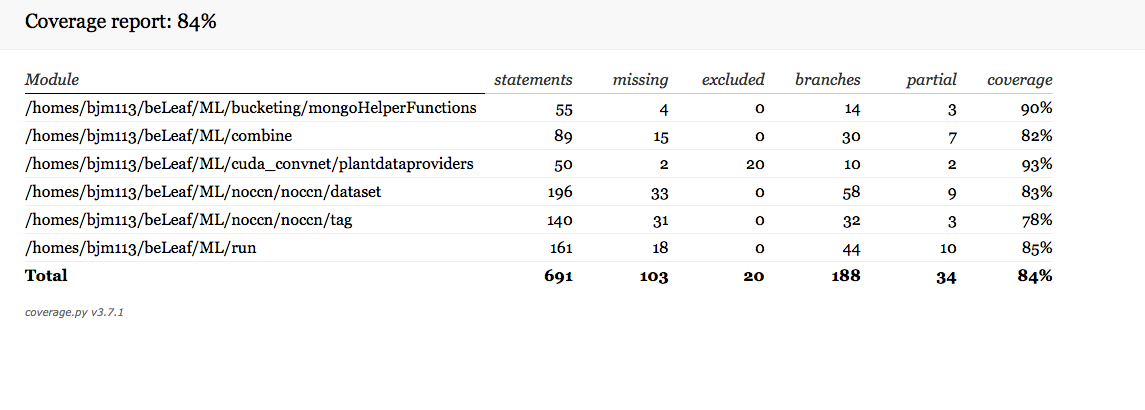
\includegraphics[width=0.7\linewidth]{ml_coverage.png}
	\caption{Sample Plant Classification Coverage Report.}
\end{figure}

\subsection{Request Server Coverage Report}
\begin{figure}[h!]
	\centering
	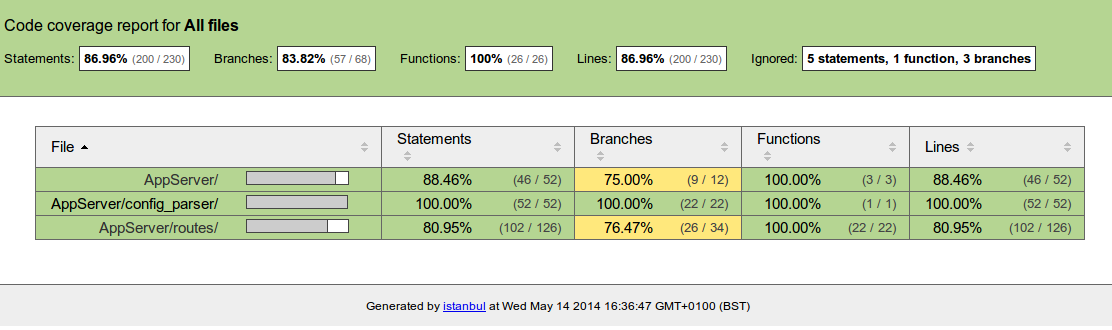
\includegraphics[width=0.7\linewidth]{request_server_coverage.png}
	\caption{Request Server Coverage Report.}
\end{figure}

\subsection{Worker Server Coverage Report}
\begin{figure}[h!]
  \centering
  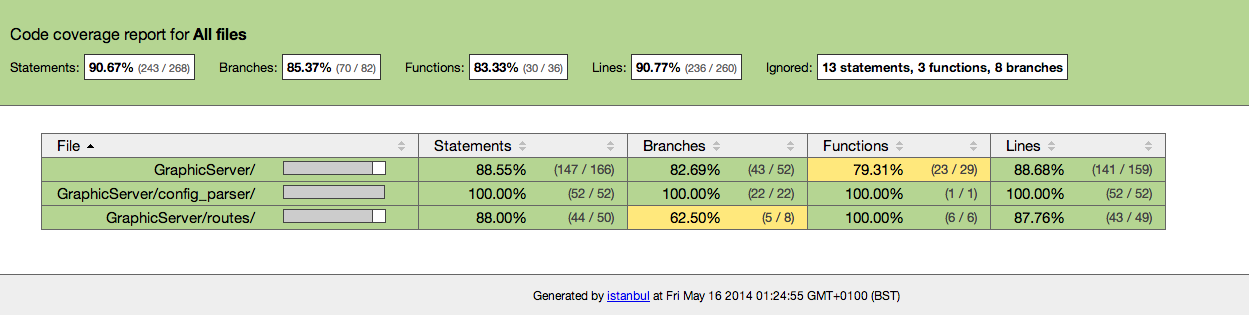
\includegraphics[width=0.7\linewidth]{worker_server_coverage.png}
  \caption{Request Server Coverage Report.}
\end{figure}

\subsection{iOS Application Unit Tests}
\begin{figure}[H]
	\centering
	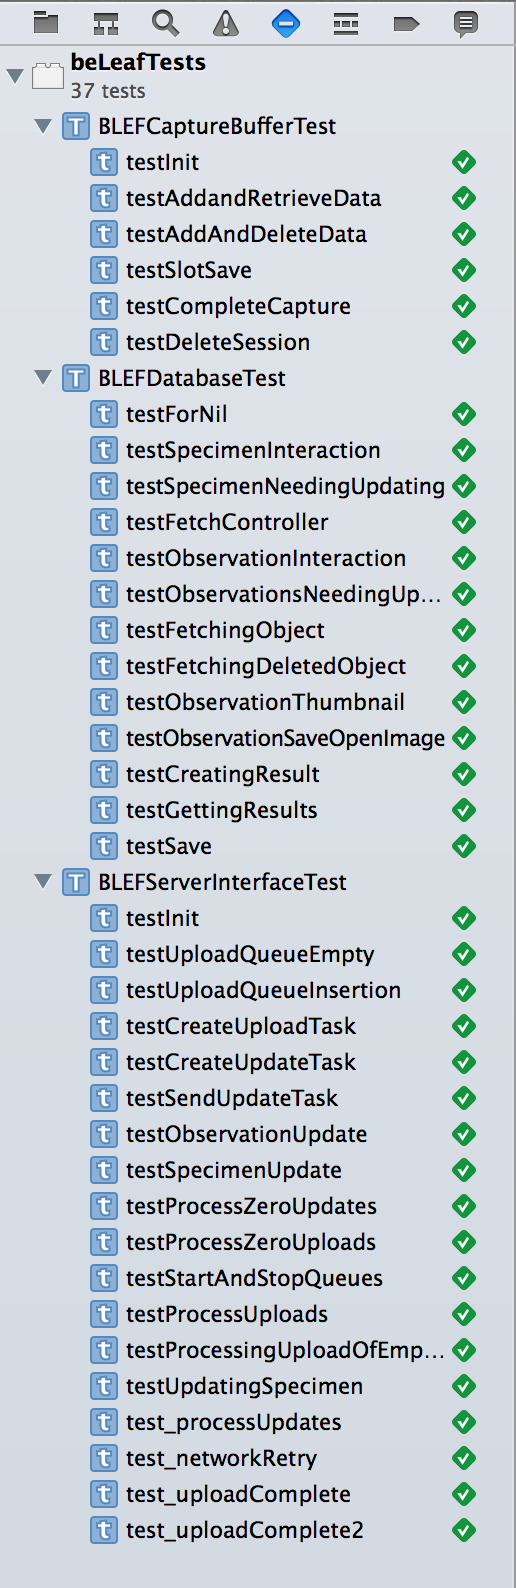
\includegraphics[width=0.3\linewidth]{images/ios_test_results.png}
	\caption{Xcode test suite.}
\end{figure}

\end{description}
\clearpage
\begin{landscape}

\section{Logbook}

\subsection{Detailed Work Breakdown}

\small
\setlength\LTleft{0pt}            % default: \parindent
\setlength\LTright{0pt}           % default: \fill
\noindent
\begin{longtable}
	{| p{1.5cm} | p{3cm} | p{3cm} | p{3cm} | p{3cm} | p{3cm} | p{3cm} | } \\ \hline
	Week Ending & Gerard & Alex & Simon & Ashley & John & Stewart \\ \hline
	24th Jan & 20 & 15 & 10 & 5 & 10 & 5 \\ \hline 
	31st Jan & 15 & 5 & 20 & 15 & 18 & 15 \\ \hline 
	7th Feb & 25 & 10 & 20 & 10 & 10 & 5 \\ \hline
	\textit{summary of work done:}
		& Wrote startup script to configure an environment with all components and optional stubs if necessary. Wrote a script to parse mocha unit test results in an email friendly way. Wrote a script to convert image meta-data from xml to json and populate a MongoDB collection. Installed necessary software on VM and graphic02	
		& Wrote a bash script that automates installation and setup of neural net to make it operable for all team members. Practiced training neural net on PlantClef images by varying parameters.	
		& Various pieces of configuration on the server (mongoDB, permissions). Implemented POST request requirement on AppServer, and linked to MongoDB. Implemented Configuration file parsing for node AppServer.	
		& Re-wrote iPhone app to have much more flexible logic and control flow. App now has custom camera view with `segment selection'.
		& Created neural network using plantclef data to categorize an image of a plant into different plant components (i.e. entire, leaf, flower, fruit, branch, stem). Wrote a tagging script which uses the above network to tag xml files corresponding to images with the component of the shot, and a batching system which takes xml data and jpgs and stores this into python pickled numpy arrays with meta-data for efficient training.	
		& Learned about node streams and integrating with databases. Tried to implement sockets. 
		\\ \hline 
	14th Feb & 20 & 15 & 15 & 20 & 20 & 15 \\ \hline
	\textit{summary of work done:}
		& Followed up with NHM re:collaboration. Increased stability of CI Server. Identified appropriate code coverage framework for NodeJs. Wrote a python script that will convert Alex's bucketing algo results into documents and insert them into MongoDB. Extended the xml2json util script to handle new logic of bucketing information being stored in MongoDB.	
		& Implemented object-oriented graph class in python to represent taxon tree. Wrote a bucketing algorithm that determines which classes can and should be classified based on number of images available and parent-child relationships, and generates a data structure optimised for mongodb querying. Tested graph building methods and added code to enforce tree structure. 
		& Improved parsing of configuration files. Implemented HTTP GET request on AppServer. Migrated AppServer to use native Mongo driver.
		& Implmented a queue processing system for the app for both uploads and result requests. After user permission promot, the location of taken photos will also collected and stored in the DB.	
		& Trained 6 (very basic) model networks for each component type (created and stored accompanying batch data also). Created a main script which takes an image and tag, loads the appropriate network (based on a config file and the tag), and outputs the probabilities of top 5 most likely species.  Also created a `test' stub equivalent for testing purposes.
		& Implemented the graphic02 node server such that it can listen for an HTTP request. Integrated John's python script. 
		\\ \hline 
	21st Feb & 10 & 0 & 10 & 10 & 15 & 10 \\ \hline
	\textit{summary of work done:} 
		& Installed and configured code coverage tool for NodeJS code. Extended startup script to start up in pseudo-dist mode and quiet mode. Continued to work on testing infrastructure	
		& 
		& Resolved mongo connection issue on graphic. Altered config files to allow pseudo-dist mode.
		& Cleaned up result page design for App Demo. Unit Test and Coverage Reports for xCode project up and running. ~98% test coverage for iOS database class attained.
		& Reviewed image data and extracted required subsets of plants from imagenet.  Created taxon tree of the plant data, with accompanying metadata. Customised tagging script for our imagenet data and tagged xml files with their component type using our trained net.	
		& Used John's python script to append JSON to the VM mongo. Exported node files to a single plant.js to allow for code coverage. 
		\\ \hline 
	28th Feb & 35 & 0 & 10 & 15 & 20 & 10 \\ \hline
	\textit{summary of work done:} 
		& wrote script to convert image meta data xml files into json, inserting them into Mongodb with appropiate wordnet columns etc. stored wordnet and taxonomy tree in mogodb(scripts provided). wore a scirpt to update the path from root to all nodes of tanonomy tree. worte bucketing algo javascript queries/functions to dynamically pull image batches from mongo for training neural nets. wrote help function script in python to facilitate interacting with mongodb and pulling in bucketed data and a function to dynamically exclude synsets from the bucketing algo.
		&  
		& Wrote unit tests for config parser. Established how to connect to mongo and how to use Istanbul and Mocha coverage and test frameworks in asynchronous manner. Wrote unit tests for server and routes (REST API) for appServer. Refactored code in server to enable easier testing.
		& Completed Unit Test coverage for App's core functinality (Database and Network Classes). Began initial structuring for the new design.	
		& Created test suite framework for machine learning modules.  Created data augmentation script with PCA analysis to mimic natural lighting changes.  Reviewed and excluded some synsets from database. Outlined and began work on combining multiple results into one classification through bayesian system. Began work on pulling bucketed classes into batching script for training a network.	
		& Began unit testing for node and started code coverage 
		\\ \hline 
	7th Mar & 10 & 10 & 15 & 30 & 25 & 15 \\ \hline
	\textit{summary of work done:} 
		& Completed unit test coverage for bucketing algo	
		& Wrote tests for augmenting data provider, creating dummy images, making sure forward increment, downward increment, flipping work.
		& Rewrote code for AppServer and adjusted database scheme to contain both group and segment collections, in order to interface correctly with the revised version of the iPhone App. Revised and added to test coverage to ensure new logic was being tested effectively.
Started to make insertions into Report2.
		& Finished moving App's UI to new design structure. Modified database and networking to be compatible with new classification architechture. App automatically continues performing network actions on launch. Added more unit tests to cover these changes.	
		& Batched image net data, and trained and supervised `one-big-net' model. Run script now stores a pickle object of the result. Batcher now creates a super set of the classes from a combination of nets and filters.  Added combine script to use a baysian optimal classifier to assemble final classification.  Added unit tests for all of the above.	
		& Updated graphic server so that, upon receiving a post request it creates a new `group' directory to save images, and updates mongo to say the segment image has been received. Began work on polling mongo for 128 images. 
		\\ \hline 
	14th Mar & 10 & 10 & 10 & 10 & 10 & 15 \\ \hline
	\textit{summary of work done:} 
		& Mostly report 2 work, and small bug fixes	
		& report 2, more work on data provider	
		& Creation of content for Report 2, draft reading, further unit tests written.	
		& Moved image-capture logic into seperate class, increasing line-count for code coverage.	
		& Built prototype templates of a smaller architecture for four separate networks.  Some minor bug fixes in the combine and run script.	
		& Created separate process, poll.js  which polls Mongo for new images in graphic and gets their location. Implemented skeleton queueing logic
		\\ \hline 
	21st Mar & 0 & 20 & 10 & 20 & 5 & 18 \\ \hline
	\textit{summary of work done:} 
		& 
		& Trained multiple versions of a leaf network, using different network architectures, dropout levels, component tagging thresholds, data augmentation hyperparameters.	
		& Testing of interaction between App and Request server. Adjustment of structure of JSON responses to restrict data being passed to iPhone to only that necessary for the results to be parsed.
		& Adding ability to change debug/production URL within the settings.app - Photos taken are center-cropped to 512x512 before being saved and uploaded. App can now generate and send notification of the `upload-session' being `completed' ready for final classification. Corrected JSON parser to conform to new result response. Many UI improvments: displays `beleaf' level as a piechart, results are ordered by confidence, proccessing results have an activity indicator. Fixed resultview scroll-bounce-bug. Tried different layout/visibility options for the camera interface.	
		& Working with the Node server to ensure the script can be run from other locations on the central graphic02 machine.	
		& Tested executing python run.py and combine.py scripts from Node server. Each group is augmented with a new field upon receipt of an image e.g. leaf: `/path/to/file', which are then combined when the user presses `upload'. Queuing logic now working satisfactorily.
		\\ \hline 
	28th Mar & 0 & 0 & 0 & 0 & 0 & 0 \\ \hline
	4th Apr & 0 & 0 & 0 & 2 & 0 & 0 \\ \hline
	\textit{summary of work done:} & & & & App sends `PUT' on user cancel & & \\ \hline 
	11th Apr & 0 & 0 & 0 & 0 & 5 & 15 \\ \hline
	\textit{summary of work done:} & & & & & Built and tried to train a network on flower components only.  Error rate was worse than that of the one big net after a week of training & Built team website using Bootstrap, including signup field to track interest \\ \hline 
	18th Apr & 0 & 0 & 0 & 0 & 20 & 0 \\ \hline
	\textit{summary of work done:} & & & & & Built a prediction suite to test the error rates by plant and overall of our nets.  Calculated network error for current network. Built a small wrapper process which keeps a single net in persistent memory and can accept request via a client process. Modified the training parameters to enlarge the test set to an arbitrary number of batches. Modified the provider classes to take random image crops and augment luminosity via pca.  Started training another big network to improve performance and test with prediction suite & \\ \hline 
	25th Apr & 0 & 0 & 0 & 5 & 0 & 0 \\ \hline
	\textit{summary of work done:} & & & & Updated UI theme & & \\ \hline 
	2nd May & 0 & 0 & 0 & 0 & 0 & 0 \\ \hline
	9th May & 0 & 0 & 0 & 2 & 0 & 0 \\ \hline
	\textit{summary of work done:} & & & & Fixed interface autolayout constrains. Add swipe-to-change-segment on camera view & & \\ \hline 
	16th May & 0 & 0 & 10 & 6 & 0 & 0 \\ \hline
	\textit{summary of work done:} & & & Updated test suite for NodeJS, ensured dependencies were locked at working versions. Created README, rationalised folder structure, adjusted Makefile. Implemented kill script for old and cancelled submissions.& Updated unit tests. Worker Server debugging session & & \\ \hline 
\end{longtable}
\end{landscape}

\clearpage

\subsection{Minutes of Group Meetings}
\lstset{breaklines=true}
\subsubsection{13/12/2013 13:00}
\lstinputlisting{./../meetingMinutes/2013_12_13-Minutes.txt}
\clearpage
\subsubsection{16/01/2014 12:00}
\lstinputlisting{./../meetingMinutes/2014_01_16-1200-Minutes.txt}
\clearpage
\subsubsection{16/01/2014 13:00}
\lstinputlisting{./../meetingMinutes/2014_01_16-1300-Minutes.md}
\clearpage
\subsubsection{17/01/2014 18:00}
\lstinputlisting{./../meetingMinutes/2014_01_17-1800-Minutes.MD}
\clearpage
\subsubsection{22/01/2014 14:00}
\lstinputlisting{./../meetingMinutes/2014_01_22-1400-Minutes.md}
\clearpage
\subsubsection{27/01/2014 15:00}
\lstinputlisting{./../meetingMinutes/2014_01_27-1500-Minutes.md}
\clearpage
\subsubsection{27/01/2014 16:30}
\lstinputlisting{./../meetingMinutes/2014_01_27-1630-Minutes.md}
\clearpage
\subsubsection{29/01/2014 14:00}
\lstinputlisting{./../meetingMinutes/2014_01_29-1400-Minutes.md}
\clearpage
\subsubsection{30/01/2014 15:00}
\lstinputlisting{./../meetingMinutes/2014_01_30-1500-Minutes.md}
\clearpage
\subsubsection{31/01/2014 10:00}
\lstinputlisting{./../meetingMinutes/2014_01_31-1000-Minutes.md}
\clearpage
\subsubsection{17/02/2014 13:00}
\lstinputlisting{./../meetingMinutes/2014_02_17-1300-Minutes.md}
\clearpage
\subsubsection{20/02/2014 15:00}
\lstinputlisting{./../meetingMinutes/2014_02_20-1500-Minutes.md}
\clearpage
\subsubsection{26/02/2014 14:00}
\lstinputlisting{./../meetingMinutes/2014_02_26-1400-UI_DESIGN_Minutes.md}
\clearpage
\subsubsection{10/03/2014 13:00}
\lstinputlisting{./../meetingMinutes/2014_03_10-1600-Minutes-Report2.md}
\clearpage
\subsubsection{12/03/2014 14:00}
\lstinputlisting{./../meetingMinutes/2014_03_12-14-Minutes-Report2-Discuss.md}
\clearpage
\subsubsection{25/03/2014 17:00}
\lstinputlisting{./../meetingMinutes/2014_03_25-1700-Minutes.md}
\clearpage
\subsubsection{12/05/2014 10:00}
\lstinputlisting{./../meetingMinutes/2014_05_12-1000-Minutes.md}
\clearpage
\subsubsection{13/05/2014 10:00}
\lstinputlisting{./../meetingMinutes/2014_05_13-1000-Minutes.md}
\lstset{breaklines=false}
\clearpage


\begin{landscape}
\subsection{Git Commit Logs}
\lstset{breaklines=true}
\lstinputlisting{./../log.txt}
\clearpage
\end{landscape}
\end{document}
